\documentclass[thesis.tex]{subfiles}

\begin{document}

\iffulldocument\else
	\chapter{KdV5}
\fi

\section{Overview}

We will construct periodic multi-pulses using Lin's method. This is an adaptation of the technique in \cite{Sandstede1997}. Rather than constructing a periodic $n$-pulse $U(x)$ as a piecewise perturbation of the primary pulse solution $Q(x)$, we take a piecewise ansatz
\[
U_i^\pm(x) = Q^\pm(x; \beta_i^\pm) + V_i^\pm(x),
\]
where the functions $Q^\pm(x; \beta_i^\pm)$ paramaterize the stable and unstable manifolds $W^s(0)$ and $W^u(0)$ near $Q(0)$, and $V_i^\pm$ is a small remainder term. The domains of the functions $U_i^\pm(x)$ will be specified below. In other words, we use the small parameters $\beta_i^\pm$ to break the homoclinic orbit $Q(x)$, and then use Lin's method to glue the pieces together. We will show that we can find a unique piecewise solution $U_i^\pm$ which generically has $n$ jumps in the direction of $\Psi(0)$. We will derive expressions for these $n$ jumps. A periodic multi-pulse solution exists if and only if these $n$ jumps are all 0.

\section{Piecewise ansatz}

First, we write $W^u(0)$ and $W^s(0)$ as graphs over their tangent spaces near $Q(0)$. Following \cite{Sandstede1997}, we can parameterize the unstable and stable manifolds near $Q(0)$ by the smooth functions $Q^-(\gamma, \beta^-)$ and $Q^+(\gamma, \beta^+)$, where $\gamma \in \R$, $\beta^\pm \in Y^\pm$ and these functions are chosen so that $Q^+(\gamma, 0) - Q^-(\gamma, 0) \in \R \Psi(0)$. Note that $Q^+(0, 0) = Q^-(0, 0) = Q(0)$. We will always take $\gamma = 0$. Using this parameterization, let
\begin{equation}\label{defQpm}
\begin{aligned}
Q^-(x; \beta^-) && x \leq 0 \\
Q^+(x; \beta^-) && x \geq 0
\end{aligned}
\end{equation}
be the unique solutions to \eqref{genODE} on $\R^\pm$ with initial conditions $Q^\pm(0, \beta^\pm)$ at $x = 0$. Since the initial conditions lie on the unstable and stable manifolds (respectively), the functions \cref{defQpm} decay exponentially (in the appropriate direction) with rate $\alpha_0$.

We will look for a $n-$periodic solution $U(n)$ to \eqref{genODE} which is piecewise of the form
\begin{equation}\label{Upiecewise}
\begin{aligned}
U_i^-(x) &= Q^-(x; \beta_i^-) + V_i^-(x) && x \in [-X_{i-1}, 0] \\
U_i^+(x) &= Q^+(x; \beta_i^+) + V_i^+(x) && x \in [0, X_i]
\end{aligned}
\end{equation}
for $i = 0, \dots, n-1$, where $U_i^-: [-X_{i-1}, 0] \rightarrow \R$ and $U_i^+: [0, X_i] \rightarrow \R$ are continuous, and the subscripts $i$ are taken $\Mod n$ since we are on a periodic domain. Essentially, we are describing $U$ by $2n$ constants $\beta_i^\pm$, representing initial conditions on the unstable and stable manifolds, and $2n$ remainder functions $V_i^\pm(x)$. Since the initial conditions of $Q^\pm(x; \beta_i^\pm)$ are in $\R Q'(0) \oplus Y^\pm$, we are free to choose $V_i^\pm(x)$ with initial conditions
\begin{align*}
V_i^-(0) &\in \R \Psi(0) \oplus Y^- \\
V_i^+(0) &\in \R \Psi(0) \oplus Y^+
\end{align*}
Since a perioidic must be continuous, in order to construct a periodic $n$-pulse, we must join the $2n$ pieces $U_i^\pm(x)$ end-to-end in a loop. Thus we need to solve the following system of equations for $i = 0, \dots, n-1$.
\begin{align}
(U_i^\pm(x))' - F(U_i^\pm(x)) &= 0 \label{exsystem1} \\
U_i^+(X_i) - U_{i+1}^-(-X_i) &= 0 \label{exsystem2} \\
U_i^+(0) - U_i^-(0) &= 0 \label{exsystem3}
\end{align}
Equation \cref{exsystem2} is a matching condition at the pulse tails, and equation \cref{exsystem3} is a matching condition at the pulse centers.

\section{Exponential Dichotomy}\label{sec:existdichot}

Let $\Phi_\pm(x, y; \beta^\pm)$ be the family of evolution operators for the ODEs
\begin{align}\label{qpmODEs}
(V^\pm(x))' &= D F\left(Q^\pm(x, \beta^\pm)\right) V^\pm(x) && x \in \R^\pm
\end{align}
By \cref{hypeqhyp}, $DF(0)$ is hyperbolic, and $|\Re \nu| \geq \alpha_0$ for all eigenvalues $\nu$ of $DF(0)$. Choose any $\alpha$ slightly smaller than $\alpha_0$. 

In the next lemma, we decompose these evolution operators in exponential dichotomies on $\R^+$ and $\R^-$. 

% lemma : exp dichotomy
\begin{lemma}\label{dichotomy1}
There exist projections
\begin{align*}
&P_+^s(y; \beta^+) && y \geq 0 \\
&P_+^u(y; \beta^+) = I - P_+^s(y; \beta^+) && y \geq 0 \\
&P_-^u(y; \beta^-) && y \leq 0 \\
&P_-^s(y; \beta^-) = I - P_-^u(y; \beta^-) && y \leq 0 \\
\end{align*}
such that the evolution operators $\Phi_\pm(x, y; \beta^\pm)$ can be decomposed as
\begin{align*}
\Phi^s_\pm(x, y; \beta^\pm) &= \Phi_\pm(x, y; \beta^\pm) P^s_\pm(y; \beta^\pm) \\
\Phi^u_\pm(x, y; \beta^\pm) &= \Phi_\pm(x, y; \beta^\pm) P^u_\pm(y; \beta^\pm) 
\end{align*}
where we have the estimates
\begin{align*}
|\Phi^s_+(x, y, \beta^+)| &\leq C e^{-\alpha(x - y)} && 0 \leq y \leq x \\
|\Phi^u_+(x, y, \beta^+)| &\leq C e^{-\alpha(y - x)} && 0 \leq x \leq y \\
|\Phi^u_-(x, y, \beta^-)| &\leq C e^{-\alpha(y - x)} && 0 \geq y \geq x \\
|\Phi^s_-(x, y, \beta^-)| &\leq C e^{-\alpha(x - y)} && 0 \geq x \geq y \\
\end{align*}
which also hold for derivatives with respect to the initial conditions $\beta^\pm$. In addition, the projections satisfy the commuting relations
\begin{align*}
\Phi_\pm(x, y; \beta^\pm) P^{s/u}_\pm(y; \beta^\pm) 
= P^{s/u}_\pm(x; \beta^\pm) \Phi_\pm(x, y; \beta^\pm)
\end{align*}
Finally, the projections can be chosen such that at $y = 0$ we have, independent of $\beta^+$ and $\beta^-$
\begin{align*}
\ker P^s_+(0; \beta^+) &= \R \Psi(0) \oplus Y^- \\
\ker P^u_-(0; \beta^-) &= \R \Psi(0) \oplus Y^+ \\
\ran P^u_+(0; \beta^+) &= \R \Psi(0) \oplus Y^- \\
\ran P^s_-(0; \beta^-) &= \R \Psi(0) \oplus Y^+
\end{align*}

\begin{proof}
Since $DF(0)$ is hyperbolic by Hypothesis \ref{hypeqhyp}, this follows from Lemma 5.1 in \cite{Sandstede1997}, which follows from Lemma 1.1 in \cite{Sandstede1993}.
\end{proof}
\end{lemma}

Let $E_0^s$ and $E_0^u$ be the stable and unstable eigenspaces of $DF(0)$, and let $P_0^s$ and $P_0^u$ be the corresponding eigenprojections. The next lemma provides a bound on the difference between the exponential dichotomy projections and the projections onto the stable and unstable eigenspaces of $DF(0)$. Essentially, the exponential dichotomy projections decay exponentially to the eigenprojections as $x \rightarrow \pm \infty$.

% lemma : bound on projection difference

\begin{lemma}\label{projdifflemma}
We have the following estimates
\begin{equation}\label{projdiffest}
\begin{aligned}
|P^u_+(x; \beta^+) - P_0^u| &\leq C e^{-\alpha x} \\
|P^s_+(x; \beta^+) - P_0^s| &\leq C e^{-\alpha x} \\
|P^u_-(x; \beta^-) - P_0^u| &\leq C e^{\alpha x} \\
|P^s_-(x; \beta^-) - P_0^s| &\leq C e^{\alpha x} 
\end{aligned}
\end{equation}
The estimates are independent of $\beta_i^\pm$.
\begin{proof}
This follows from Lemma 1.1 and Lemma 2.1 in \cite{Sandstede1993}.
\end{proof}
\end{lemma}

\section{Fixed Point Formulation}

In this section, we formulate equation \eqref{exsystem1} as a fixed point problem. First, we plug in the piecewise ansatz \eqref{Upiecewise} into \eqref{genODE}. For $i = 0, \dots, n-1$, we have 
\begin{align*}
U_i^\pm(x)' &= (Q^\pm(x; \beta_i^\pm))' + V_i^\pm(x)' = F\left(Q^\pm(x; \beta_i^\pm) + V_i^\pm(x) \right) \\
\end{align*}
Since $Q^\pm(x; \beta_i^\pm)$ solves \eqref{genODE} on $\R^\pm$, 
\begin{align*}
(V_i^\pm(x))' &= F\left(Q^\pm(x; \beta_i^\pm) + V_i^\pm(x) \right) - F(Q^\pm(x; \beta_i^\pm))
\end{align*}
Expanding the RHS in a Taylor series (using the version for Banach spaces) about $Q^\pm(x; \beta_i^\pm)$, we attain the ODE for $V_i^\pm$.
\begin{equation}\label{Vpiecewise}
(V_i^\pm(x))' = DF(Q^\pm(x; \beta_i^\pm)) V_i^\pm(x) + G_i^\pm(x; \beta_i^\pm, V_i^\pm)
\end{equation}
where 
\begin{equation}\label{Gquadratic}
G_i^\pm(\beta_i^\pm, V_i^\pm)(x) = \mathcal{O}(|V_i^\pm|^2)
\end{equation}
This estimate is independent of the parameters $\beta_i^\pm$ since we can get a uniform bound for $Q^\pm(0, \beta_i^\pm)$ for sufficiently small $\beta_i^\pm$. As in \cite{Sandstede1997}, derivatives of $G_i^\pm$ with respect to the parameters $\beta_i^\pm$ are the same order in $V_i^\pm$.

We now rewrite the piecewise differential equations \eqref{Vpiecewise} in integrated form to get the fixed point equations.
\begin{equation}\label{FPequations}
\begin{aligned}
V_i^+(x) &= \Phi^u_+(x, X_i; \beta_i^+) a_i^+  \\
&+ \int_{X_i}^x \Phi_+^u(x, y; \beta_i^+) G_i^+(y; V_i^+(y),\beta_i^+)dy \\
&+ \int_0^x \Phi_+^s(x, y; \beta_i^+) G_i^+(y; V_i^+(y),\beta_i^+)dy \\ 
V_i^-(x) &= \Phi^s_-(x, -X_{i-1}; \beta_i^-) a_{i-1}^-  \\
&+ \int_{-X_{i-1}}^x \Phi_-^s(x, y; \beta_i^-) G_i^-(y; V_i^-(y),\beta_i^-)dy \\
&+ \int_0^x \Phi_-^u(x, y; \beta_i^-) G_i^-(y; V_i^-(y),\beta_i^-)dy \\
\end{aligned}
\end{equation}
where for the initial conditions $a_i^\pm$ at $-X_{i-1}$ and $X_i^+$, we take $a_i^+ \in E_0^u$ and $a_i^- \in E_0^s$. We do not have initial conditions at $x = 0$ for the other half of the dichotomy since those initial conditions are incorporated into $\beta_i^\pm$.

Finally, define the exponentially weighted norms
\begin{equation}\label{expwtnorm}
\begin{aligned}
||V||_{X, +} &= \sup_{x \in [0, X]} e^{\alpha(X - x)}|V(x)| \\
||V||_{X, -} &= \sup_{x \in [-X, 0]} e^{\alpha(X + x)}|V(x)|
\end{aligned}
\end{equation}
Let $K_{X, \pm}$ be the Banach spaces of continuous functions on $[0, X]$ and $[-X, 0]$ equipped with these norms. Let $B_{X, \pm}(\rho)$ be the ball of radius $\rho$ about $0$ in these spaces.

\section{Inversion}

As in \cite{SandstedeStrut}, we will solve for the remainder functions $V_i^\pm$ and initial conditions $\beta_i^\pm$ in a series of lemmas. First, we will solve equation \cref{exsystem1} for the $V_i^\pm(x)$ in terms of the initial conditions $a_i^\pm$. Note that $V_i^+(x)$ only depends on $a_i^+$ and $V_i^-(x)$ only depends on $a_{i-1}^-$.

% lemma : solve for V_i^\pm

\begin{lemma}\label{solveforV}
There exist $\delta, \rho > 0$ such that for $|X_i|, |X_{i-1}| > 1/\delta$ and $|a_{i-1}^-|, |a_i^+|, |\beta_i^\pm| < \delta$, there exist unique solutions
\begin{align*}
V_i^-(a_{i-1}^-, \beta_i^-) &\in B_{X_{i-1}, -}(\rho) \\
V_i^+(a_i^+, \beta_i^+) &\in B_{X_i, +}(\rho) \\
\end{align*}
to the fixed point equations \eqref{FPequations}. $V_i^-(a_{i-1}, \beta_i^-)$ depends smoothly on $(a_{i-1}^-, \beta_i^-)$, and $V_i^+(a_i, \beta_i^+)$ depends smoothly on $(a_i^+, \beta_i^+)$. Finally, we have the estimates
\begin{equation}\label{Vest}
\begin{aligned}
||V_i^-||_{X_{i-1}, -} &\leq C |a_{i-1}^-| \\
||V_i^+||_{X_i, +} &\leq C |a_i^+|
\end{aligned}
\end{equation}
where the constant $C$ depends only on $\delta$. These estimates hold as well for derivatives of $V_i^\pm$ with respect to $\beta_i^\pm$.
\begin{proof}
The proof follows that of Lemma 5.2 in \cite{Sandstede1997}. Since we can deal with each of the $2n$ pieces separately, we will do only the pieces on $\R^+$ here; the pieces on $\R^-$ are similar.

The RHS of the fixed point equation \eqref{FPequations} on $\R^+$ defines a smooth mapping on $K_{X_i, +}$. We need to verify that the RHS maps $K_{X_i, +} \mapsto K_{X_i, +}$. To do this, we obtains bounds on three terms on the RHS individually using the estimates on $\Phi^{s/u}_\pm$ from Lemma \ref{dichotomy1}. For the first term on the RHS,
\begin{align*}
e^{\alpha(X_i - x)} | \Phi^u_+(x, X_i; \beta_i^+) a_i^+ | 
&\leq C e^{\alpha(X_i - x)} e^{-\alpha(X_i - x)} |a_i^+| \\
&\leq C |a_i^+|
\end{align*}
For the second term, we also use the estimate on $G$ from \eqref{Gquadratic}, and the fact that $V_i^+ \in K_{X_i, +}$. 
\begin{align*}
e^{\alpha(X_i - x)} &\left| \int_{X_i}^x \Phi_+^u(x, y; \beta_i^+) G_i^+(y, V_i^+(y),\beta_i^+)dy  \right| \\
&\leq C e^{\alpha(X_i - x)} \int_x^{X_i} e^{-\alpha(y - x)}|V_i^+(y)|^2 dy \\
&\leq C e^{\alpha(X_i - x)} \int_x^{X_i} 
e^{-\alpha(y - x)}(e^{-\alpha(X_i - y)})^2|e^{\alpha(X_i - y)} V_i^+(y)|^2 dy \\
&\leq C e^{\alpha(X_i - x)} \int_x^{X_i} 
e^{-\alpha(y - x)}(e^{-\alpha(X_i - y)})^2 dy \\
&\leq C \int_0^{X_i} e^{-\alpha (X_i - y)} dy \\
&\leq C
\end{align*}
The third term is similar. Thus the RHS of the fixed point equation \eqref{FPequations} on $\R^+$ is a smooth map $K_{X_i, +} \mapsto K_{X_i, +}$. 

Define $H: K_{X_i, +} \times E_0^s \rightarrow K_{X_i, +}$ by
\begin{align*}
H(V_i^+(x), a_i^+, \beta_i^+) &= V_i^+(x) - \Phi^u_+(x, X_i; \beta_i^+) a_i^+  \\
&- \int_{X_i}^x \Phi_+^u(x, y; \beta_i^+) G_i^+(y, V_i^+(y),\beta_i^+)dy \\
&- \int_0^x \Phi_+^s(x, y; \beta_i^+) G_i^+(y, V_i^+(y),\beta_i^+)dy 
\end{align*}
which is just the RHS of the fixed point equation \eqref{FPequations} on $\R^+$. Since $Q(x)$ satisfies \eqref{genODE}, $H(0, 0, 0) = 0$. Since $G$ is quadratic in $V_i^+(x)$, the Fr\'echet derivative of $H$ with respect to $V_i^+(x)$ at $(V_i^+(x), a_i^+, \beta_i^+) = (0, 0, 0)$ is the identity, thus is a Banach space isomorphism on $K_{X_i, +}$. Using the implicit function theorem, we can solve for $V_i^+(x)$ in terms of $(a_i^+, \beta_i^+)$ for sufficiently small $|a_i^+|, |\beta_i^+|$. Since the map $H$ is smooth, this dependence is smooth.

The estimate on $V_i^\pm$ comes from the estimate of the first term on the RHS of the fixed point equations, since the other terms (those involving the integrals) are quadratic in $V_i^\pm(x)$. Since the estimate \eqref{Gquadratic} on $G$ is independent of $\beta_i^\pm$, the estimate on {}$V_i^\pm$ is also independent of $\beta_i^\pm$. Since the exponential dichotomy estimates from Lemma \ref{dichotomy1} hold for derivatives with respect $\beta_i^\pm$, these estimates also hold for derivatives with respect $\beta_i^\pm$.
\end{proof}
\end{lemma}

Next, we satisfy equation \eqref{exsystem2} to match the pieces \eqref{Upiecewise} at their tails. This will solve for the initial conditions $a_i^\pm$.

% Lemma : solve for a_i^\pm

\begin{lemma}\label{solvefora}
For any $X_i$ and $\beta_i^\pm$ chosen as in Lemma \ref{solveforV}, there is a unique pair of initial conditions $(a_i^+, a_i^-) \in E_0^s \times E_0^u$ such that $U_i^+(X_i) - U_{i+1}^-(-X_i) = 0$. $(a_i^+, a_i^-)$ depends smoothly on $(\beta_i^+, \beta_{i+1}^-)$, and we have the following estimate, which is independent of $(\beta_i^+, \beta_{i+1}^-)$.
\begin{equation}\label{aest}
|a_i^\pm| \leq C e^{-\alpha X_i}
\end{equation}
This holds as well for derivatives with respect to $\beta_i^\pm$. We also have the following expressions for $a_i^\pm$.
\begin{equation}\label{aiformula}
\begin{aligned}
a_i^+ &= -P^u_0 \left( Q^+(X_i; \beta_i^+) - Q^-(-X_i; \beta_{i+1}^-) \right) + \mathcal{O}( e^{-2 \alpha X_i} ) \\
a_i^- &= P^s_0 \left( Q^+(X_i; \beta_i^+) - Q^-(-X_i; \beta_{i+1}^-) \right) + \mathcal{O}\left( e^{-2 \alpha X_i} \right)
\end{aligned}
\end{equation}

\begin{proof}
First, we plug in the fixed point equations \eqref{FPequations} to the expressions \eqref{Upiecewise} for $U_i^+$ and $U_{i+1}^-$ and evaluate them at $\pm X_i$ to get
\begin{align*}
U_i^+(X_i) &= Q^+(X_i; \beta_i^+) + P^u_+(X_i; \beta_i^+) a_i^+ \\
&+ \int_0^{X_i} \Phi_+^s(X_i, y; \beta_i^+) G_i^+(y, V_i^+(y),\beta_i^+)dy \\ 
U_{i+1}^-(-X_i) &= Q^-(-X_i; \beta_{i+1}^-) + P^s_-(-X_i; \beta_{i+1}^-) a_i^- \\
&+ \int_0^{-X_i} \Phi_-^u(-X_i, y; \beta_{i+1}^-) G_{i+1}^-(y, V_{i+1}^-(y),\beta_{i+1}^-)dy \\
\end{align*}
Adding and subtracting the projections $P_0^s$ and $P_0^u$ and recalling that $a_i^+ \in E_0^u$ and $a_i^- \in E_0^s$, this becomes
\begin{align*}
U_i^+(X_i) &= Q^+(X_i; \beta_i^+) + a_i^+ + (P^u_+(X_i; \beta_i^+) -  P^u_0)a_i^+ \\
&+ \int_0^{X_i} \Phi_+^s(X_i, y; \beta_i^+) G_i^+(y, V_i^+(y),\beta_i^+)dy \\ 
U_{i+1}^-(-X_i) &= Q^-(-X_i; \beta_{i+1}^-) + a_i^- + (P^s_-(-X_i; \beta_{i+1}^-) - P^s_0) a_i^- \\ 
&+ \int_0^{-X_i} \Phi_-^u(-X_i, y; \beta_{i+1}^-) G_{i+1}^-(y, V_{i+1}^-(y),\beta_{i+1}^-)dy
\end{align*}
Subtract these to get $H: E_0^s \times E_0^u \times \R \times \R \rightarrow \R^{2m}$, defined by
\begin{align*}
H(a_i^+, &a_i^-, \beta_i^+, \beta_{i+1}^-) 
= a_i^+ - a_i^- + (P^u_+(X_i; \beta_i^+) -  P^u_0)a_i^+ - (P^s_-(-X_i; \beta_{i+1}^-) - P^s_0) a_i^-  \\
&+ Q^+(X_i; \beta_i^+) - Q^-(-X_i; \beta_{i+1}^-)\\
&+ \int_0^{X_i} \Phi_+^s(X_i, y; \beta_i^+) G_i^+(y, V_i^+(y),\beta_i^+)dy
- \int_0^{-X_i} \Phi_-^u(-X_i, y; \beta_{i+1}^-) G_{i+1}^-(y, V_{i+1}^-(y),\beta_{i+1}^-)dy 
\end{align*}
We need to solve $H(a_i^+, a_i^-, \beta_i^+, \beta_{i+1}^-) = 0$ for $a_i^\pm$. Plugging in the solution for $V_i^\pm(x)$ from Lemma \ref{solveforV}, this becomes
\begin{align*}
H(a_i^+, &a_i^-, \beta_i^+, \beta_{i+1}^-) \\
&= a_i^+ - a_i^- + (P^u_+(X_i; \beta_i^+) -  P^u_0)a_i^+ - (P^s_-(-X_i; \beta_{i+1}^-) - P^s_0) a_i^-  \\
&+ Q^+(X_i; \beta_i^+) - Q^-(-X_i; \beta_{i+1}^-) \\
&+ \int_0^{X_i} \Phi_+^s(X_i, y; \beta_i^+) G_i^+(y, V_i^+(a_i^+, \beta_i^+)(y),\beta_i^+)dy \\
&- \int_0^{-X_i} \Phi_-^u(-X_i, y; \beta_{i+1}^-) G_{i+1}^-(y, V_{i+1}^-(a_i^-, \beta_{i+1}^-)(y),\beta_{i+1}^-)dy 
\end{align*}

Again, since $Q(x)$ satisfies \eqref{genODE}, $H(0, 0, 0, 0) = 0$. To  solve for $a_i^\pm$ using the implicit function theorem, we need to evaluate $D_{a_i^\pm} H(0, 0, 0, 0)$. When we take the partial derivatives with respect to $a_i^\pm$ at $a_i^\pm = 0$, the derivatives of the integral terms will be 0 since $G_i^\pm$ is quadratic order in $V_i^\pm$, thus quadratic order in $a_i^\pm$ by Lemma \ref{solveforV}. The $Q^\pm$ terms do not involve $a_i^\pm$. Using the estimate \eqref{projdiffest} from Lemma \ref{projdifflemma}, we have 
\[
\frac{\partial}{\partial a_i^\pm} H(0, 0, 0, 0) = \pm 1 + \mathcal{O} (e^{-\alpha X_i})
\]
For sufficiently large $X_i$, $D_{a_i^\pm} H(0, 0, 0, 0)$ is invertible in a neighborhood of $(0, 0, 0, 0)$. Thus we can use the IFT to solve for $a_i^\pm$ in terms of $\beta_i^\pm$. 

To obtain an expression and estimates for the $a_i^\pm$, we apply the projections $P^u_0$ and $P^s_0$ in turn to $H(a_i^+, a_i^-, \beta_i^+, \beta_{i+1}^-) = 0$. Using $P^u_0$, we have
\begin{equation}\label{Ps0aiplus}
\begin{aligned}
0 &= a_i^+ + P^u_0(P^u_+(X_i; \beta_i^+) -  P^u_0)a_i^+ 
+ P^u_0 \left( Q^+(X_i; \beta_i^+) - Q^-(-X_i; \beta_{i+1}^-) \right)\\
&+ P^u_0 \left( \int_0^{X_i} \Phi_+^s(X_i, y; \beta_i^+) G_i^+(y, V_i^+(a_i^+, \beta_i^+)(y),\beta_i^+)dy \right) \\
&- P^u_0 \left( \int_0^{-X_i} \Phi_-^u(-X_i, y; \beta_{i+1}^-) G_{i+1}^-(y, V_{i+1}^-(a_i^-, \beta_{i+1}^-)(y),\beta_{i+1}^-) dy \right)
\end{aligned}
\end{equation}
We can get estimates for all of these terms. For the first term, we use the estimate \eqref{projdiffest} from Lemma \ref{projdifflemma} to get 
\begin{align*}
|P^u_0(P^u_+(X_i; \beta_i^+) -  P^u_0)a_i^+ | &\leq C e^{-\alpha X_i} |a_i^+|
\end{align*}
For the second term, we use the decay rates of $Q^\pm$ to get
\begin{align*}
|P^u_0 \left( Q^+(X_i; \beta_i^+) - Q^-(-X_i; \beta_{i+1}^-)  \right)| &\leq C e^{-\alpha X_i}
\end{align*}
For the integral terms, we use Lemma \ref{solveforV} to get
\begin{align*}
\left| \int_0^{X_i} \Phi_+^s(X_i, y; \beta_i^+) G_i^+(y, V_i^+(a_i^+, \beta_i^+)(y),\beta_i^+)dy \right| &\leq C \int_0^{X_i}e^{-\alpha(X_i - y)} |V_i^+(y)|^2 dy \\
&\leq C \int_0^{X_i}e^{-3 \alpha (X_i - y)} |e^{\alpha(X_i - y)} V_i^+(y)|^2 dy \\
&\leq C \int_0^{X_i}e^{-3 \alpha (X_i - y)} (||V_i^+||_{X_i, +})^2 dy \\
&\leq C |a_i^+|^2
\end{align*}
The other integral term is similar. Substituting these estimates into \eqref{Ps0aiplus}, we get
\begin{align*}
|a_i^+|\left(1 + \mathcal{O}(e^{-\alpha X_i} + |a_i^+|) \right) =  
\mathcal{O}( e^{-\alpha X_i} )
\end{align*}
Thus for sufficiently large $X_i$, 
\[
|a_i^+| \leq C e^{-\alpha X_i}
\]
Using this bound together with the bounds we already have, equation \eqref{Ps0aiplus} becomes
\begin{align*}
a_i^+ &= -P^u_0 \left( Q^+(X_i; \beta_i^+) - Q^-(-X_i; \beta_{i+1}^-) \right) 
+ \mathcal{O}\left( e^{-\alpha X_i} |a_i^+| + |a_i^+|^2 \right) \\
&= -P^u_0 \left( Q^+(X_i; \beta_i^+) - Q^-(-X_i; \beta_{i+1}^-) \right) 
+ \mathcal{O}\left( e^{-2 \alpha X_i} \right)
\end{align*}
We obtain the estimate and expression for $a_i^-$ in a similar way by using the projection $P_0^s$.
\end{proof}
\end{lemma}

It only remains to satisfy equation \eqref{exsystem3}, i.e. $U_i^+(0) = U_i^-(0)$, which will match the pieces \eqref{Upiecewise} at $x = 0$. In other words, we need to solve
\begin{align}\label{Umatchat0}
V_i^+(0) - V_i^-(0) + Q^+(0; \beta_i^+) - Q^-(0; \beta_i^-) &= 0  && i = 0, \dots, n-1
\end{align}
Before we can do that, we will need to make a smooth change of coordinates near $Q(0)$ by using a variation of the flow-box method to ``straighten out'' the stable and unstable manifolds near $Q(0)$ so that their non-intersecting directions are $Y^+$ and $Y^-$.

% lemma : straighten out manifolds

\begin{lemma}\label{straightenW}
There exists a differentiable map $S: \R \times Y^- \times Y^+ \times \R\Psi(0) \rightarrow \R^{2m}$ such that $S(0, 0, 0, 0) = Q(0)$, $S$ is invertible in a neighborhood of $Q(0)$, and
\begin{align*}
S^{-1}(Q^-(0; \beta^-)) &= \beta^- \in Y^- \\
S^{-1}(Q^+(0; \beta^+)) &= \beta^+ \in Y^+ \\
\end{align*}
for sufficiently small $\beta^\pm$.
\begin{proof}
$Q'(0) = F(Q(0)) \neq 0$, i.e. the center of the primary pulse is not an equilibrium of the vector field $F$. Recall that $\R^{2m} = \R Q'(0) \oplus Y^+ \oplus Y^- \oplus \R \Psi(0)$. Let $\Theta_x(P)$ be the solution operator for \eqref{genODE}, i.e. the operator which takes an initial condition $P$ and maps it to the point $U(x)$, where $U$ is the unique solution to \eqref{genODE} with $U(0) = P$. Define the map $S: \R \times Y^- \times Y^+ \times \Psi(0) \rightarrow \R^{2m}$ by 
\begin{equation}\label{flowboxdefS}
S(x; \beta^-, \beta^+, \gamma) = \Theta_x\left(Q(0) + Q^-(0; \beta^-) + Q^-(0; \beta^+) + \gamma \Psi(0)\right)
\end{equation}
In other words, $S(y; \beta^-, \beta^+, \gamma)$ is a trajectory of \eqref{genODE} with initial condition $Q(0) + Q^-(0; \beta^-) + Q^-(0; \beta^+,0) + \gamma \Psi(0)$. For small $x, \beta^\pm$ the stable and unstable manifolds are the surfaces
\begin{align*}
W^u &= S(x; \beta^-, 0, 0) \\
W^s &= S(x; 0, \beta^+, 0) 
\end{align*}
Their one-dimensional intersection is the homoclinic orbit $Q(x) = S(x; 0, 0, 0)$, whose tangent space is $Q'(x)$. In particular, $S(0, 0, 0, 0) = Q(0)$.

To complete the proof, we need to show that $S$ is invertible in a neighborhood of the origin. For the Jacobian of $S$ at the origin, we have the following partial derivatives
\begin{align*}
S_x(0, 0, 0, 0) &= F(Q(0)) = Q'(0) \\
S_{\beta^-}(0, 0, 0, 0) &= (Q^-)_{\beta^-}(0; 0) = Y^- \\
S_{\beta^+}(0, 0, 0, 0) &= (Q^+)_{\beta^+}(0; 0) = Y^+ \\
S_{\gamma}(0, 0, 0, 0) &= \Psi(0)
\end{align*}
Since $\R^{2m} = \R Q'(0) \oplus Y^+ \oplus Y^- \oplus R \Psi(0)$, the four partial derivatives of $S$ at the origin are linearly independent, thus the Jacobian of $S$ at the origin is invertible. By the inverse function theorem, there exists open neighborhoods $N_1$ of 0 and $N_2$ of $Q(0)$ such that $S(N_1) = N_2$ and $S$ is invertible on $N_2$. In particular, for sufficiently small $\beta^\pm$
\begin{align*}
S^{-1}(Q^-(0; \beta^-) &= \beta^- \in Y^- \\
S^{-1}(Q^+(0; \beta^+) &= \beta^+ \in Y^+ \\
\end{align*}
\end{proof}
\end{lemma}

Before we solve the matching conditions \eqref{Umatchat0} at $x = 0$, we change coordinates near $Q(0)$ according to Lemma \ref{straightenW}. In the ``straightened out'' coordinates, \eqref{genODE} becomes
\begin{equation}\label{straightenedODE}
\tilde{U}' = DS(S^{-1}(\tilde{U})) F( S^{-1}(\tilde{U}) )
\end{equation}
where $S$ is defined in Lemma \ref{straightenW}. If we match $\tilde{U}_i^\pm(x)$ at $x = 0$, then since $S^{-1}$ is a homeomorphism near $Q(0)$, we have also matched $U_i^\pm(x)$ at $x = 0$. For convenience of notation, we will continue to write the transformed ODE \eqref{straightenedODE} as $U' = F(U)$ after the coordinate change.

Since $\R^{2m} = \R Q'(0) \oplus Y^+ \oplus Y^- \oplus \R \Psi(0)$, we will solve the matching conditions $U_i^+(0) - U_i^-(0) = 0$ by projecting \eqref{Umatchat0} onto these subspaces and solving separately on each subspace. Because of the coordinate change near $Q(0)$,
\begin{equation}\label{projQpm}
\begin{aligned}
P_{\R Q'(0)}(Q^\pm(0; \beta^\pm)) &= 0 \\
P_{Y}(Q^\pm(0; \beta^\pm)) &= \beta^\pm \\
P_{\R \Psi(0)}(Q^\pm(0; \beta^\pm)) &= 0
\end{aligned}
\end{equation}
where $Y = Y^+ \oplus Y^-$. Since $V_i^\pm(0) \in \R \Psi(0) \oplus Y$, the projection on $\R Q'(0)$ is always 0. Thus we only need to solve the equations
\begin{align*}
P_{Y}(U_i^+(0) - U_i^-(0)) &= 0 \\
P_{\R \Psi(0)}(U_i^+(0) - U_i^-(0)) &= 0
\end{align*}
Substituting \eqref{Upiecewise} for $U_i^\pm$ and using \eqref{projQpm}, these equations become
\begin{align}
P_{Y}(V_i^+(0) - V_i^-(0)) + (\beta_i^+ - \beta_i^-) &= 0 \label{PYmatch} \\
P_{\R \Psi(0)}(V_i^+(0) - V_i^-(0)) &= 0 \label{PZmatch}
\end{align}

We will solve these in turn. In the next lemma we solve \eqref{PYmatch} to get $(\beta_i^+, \beta_i^-)$, $i = 0, \dots, n-1$.

% lemma : solve for the \beta_i^\pm

\begin{lemma}\label{solveforbeta}
For $i = 0, \dots, n-1$, there exist $(\beta_i^+, \beta_i^-)$ such that $P_{Y^\pm}(U_i^+(0) - U_i^-(0)) = 0$. In addition, we have the estimates
\begin{equation}\label{betaest}
\begin{aligned}
|\beta_i^+| &\leq C e^{-2 \alpha X_{i-1}} \\
|\beta_i^-| &\leq C e^{-2 \alpha X_i}
\end{aligned}
\end{equation}
\begin{proof}
Substitute the fixed point equations \eqref{FPequations} evaluated at $x = 0$ into \eqref{PYmatch} to get
\begin{equation}\label{PYmatch1}
\begin{aligned}
0 &= \beta_i^+ - \beta_i^- \\
&+ P_{Y^\pm} \left( \Phi^u_+(0, X_i; \beta_i^+) a_i^+ 
+ \int_{X_i}^0 \Phi_+^u(0, y; \beta_i^+) G_i^+(y, V_i^+(y),\beta_i^+)dy \right) \\
&- P_{Y^\pm} \left( \Phi^s_-(0, -X_{i-1}, \beta_i^-) a_{i-1}^- 
+ \int_{-X_{i-1}}^0 \Phi_-^s(0, y, \beta_i^-) G_i^-(y, V_i^-(y),\beta_i^-) dy \right) 
\end{aligned}
\end{equation}
From Lemma \ref{dichotomy1}, since $\text{Ran }P_+^u(0; \beta^+) = \R \Psi(0) \oplus Y^-$, the terms involving $\Phi^u_+$ can have no component in $Y^+$. Similarly, since $\text{Ran }P_-^s(0; \beta^-) = \R \Psi(0) \oplus Y^+$, the terms involving $\Phi^s_-$ can have no component in $Y^-$. Thus it makes sense to separate \eqref{PYmatch1} into the individual projections on $Y^-$ and $Y^+$. Define $H: Y^+ \oplus Y^- \rightarrow Y^+ \oplus Y^-$ by
\begin{equation}\label{defHPY}
H(\beta_i^+, \beta_i^-) = 
\begin{pmatrix}
\beta_i^+ - P_{Y^+}\left(\Phi^s_-(0, -X_{i-1}, \beta_i^-) a_{i-1}^- 
- \int_{-X_{i-1}}^0 \Phi_-^s(0, y, \beta_i^-) G_i^-(y, V_i^-(y),\beta_i^-) dy\right) \\
\beta_i^- + P_{Y^-}\left( \Phi^u_+(0, X_i; \beta_i^+) a_i^+ 
+ \int_{X_i}^0 \Phi_+^u(0, y; \beta_i^+) G_i^+(y, V_i^+(y),\beta_i^+)dy \right)
\end{pmatrix}
\end{equation}
Note that $\beta_i^+$ and $\beta_i^+$ appear in both equations on the RHS. Using the estimates from Lemmas \ref{dichotomy1}, \ref{solveforV}, and \ref{solvefora},
\begin{equation}\label{H0bound}
H(0,0) = \mathcal{O}\left( e^{-2 \alpha X_{i-1}} + e^{-2 \alpha X_i}\right)
\end{equation}
which is independent of $\beta_i^\pm$. We would like to use the inverse function theorem to solve $H(\beta_i^+, \beta_i^-) = 0$ for $(\beta_i^+, \beta_i^-)$. To find the Jacobian, we will evaluate the partial derivatives with respect to $\beta_i^\pm$. Before we do that, recall that we solved for $V_i^\pm(x)$ and $a_i^\pm$ in Lemmas \ref{solveforV} and \ref{solvefora}, so we first plug in those solutions. For the partial derivatives of the terms involving $a_i^\pm$, we have
\begin{align*}
\left| \frac{\partial}{\partial \beta_i^+} \Phi^u_+(\beta_i^+, 0, X_i) a_i^+ \right| \leq C e^{-\alpha X_i}|a_i^+|
& \leq C e^{-2 \alpha X_i}
\end{align*}
where we used the estimate \eqref{aest} for $|a_i^+|$ and the exponential dichotomy estimates from Lemma \ref{dichotomy1}, which also apply for derivatives with respect to $\beta_i^+$. The partial derivative with respect to $\beta_i^-$ is similar, except it involves $X_{i-1}$. For the integral terms, 
\begin{align*}
\left| \frac{\partial}{\partial \beta_i^-} \int_{-X_{i-1}}^0 \Phi_-^s(\beta_i^-, 0, y) G^-(y, V^-(y),\beta^-)dy \right| 
&\leq C \int_{-X_{i-1}}^0 e^{\alpha y} | V_i^-(y) |^2 dy \\
&\leq C \int_{-X_{i-1}}^0 e^{\alpha y} | a_i^-|^2 dy \\
&\leq C e^{-2 \alpha X_{i-1}}
\end{align*}
where we used the estimates \eqref{Vest} and \eqref{aest} for $V_i^\pm$ and $a_i^\pm$. The other integral terms are similar.

Putting all of this together, the Jacobian of $H$ is given by
\begin{equation}
D H(\beta_i^+, \beta_i^-) = 
\begin{pmatrix}
1 & \mathcal{O}(e^{-2 \alpha X_{i-1}} ) \\
\mathcal{O}(e^{-2 \alpha X_i}) &  1 
\end{pmatrix}
\end{equation}
This has determinant $1 + \mathcal{O}(e^{-2\alpha (X_i+X_{i-1}})$, so is invertible for sufficiently large $X_i$. Using the inverse function theorem, we can invert $H$ in a neighborhood of $(\beta_i^+, \beta_i^-) = (0, 0)$. Specifically, there exist neighborhoods $U_1$ of $(0,0)$ and $U_2$ of $H(0,0)$ such that $H: U_1 \rightarrow U_2$ is invertible. Using \eqref{H0bound}, for sufficiently large $X_i$, the neighborhood $U_2$ will contain $(0,0)$. Thus the unique solution to $H(\beta_i^+, \beta_i^-) = 0$ is given by
\[
(\beta^+, \beta^-) = H^{-1}(0, 0)
\]
Using \eqref{defHPY} and the estimates from Lemmas \ref{dichotomy1}, \ref{solveforV}, and \ref{solvefora}, we obtain estimates
\begin{align*}
|\beta_i^+| &\leq C e^{-2 \alpha X_{i-1}} \\
|\beta_i^-| &\leq C e^{-2 \alpha X_i}
\end{align*}
\end{proof}
\end{lemma}

We have found a unique solution to \eqref{exsystem1} and \eqref{exsystem2} such that \eqref{exsystem3} is satisfied except for $n$ jumps in the direction of $\Psi(0)$. We summarize what we have obtained so far in the following lemma, which also provides bounds on the remainder terms.

% bounds in this lemma

\begin{lemma}\label{solvewithjumps}
There exists $X^* > 0$ such that for $|X_i| \geq X^*$, $i = 0, \dots, n-1$, there are unique solutions
\begin{equation*}
\begin{aligned}
U_i^-(x) &= Q^-(x; \beta_i^-) + V_i^-(x) && x \in [-X_{i-1}, 0] \\
U_i^+(x) &= Q^+(x; \beta_i^+) + V_i^+(x) && x \in [0, X_i]
\end{aligned}
\end{equation*}
to the system of equations
\begin{equation}\label{systemwithjumpZ}
\begin{aligned}
(U_i^\pm(x))' - F(U_i^\pm(x)) &= 0 \\
U_i^+(X_i) - U_{i+1}^-(-X_i) &= 0 \\
U_i^+(0) - U_i^-(0) &\in \R \Psi(0)
\end{aligned}
\end{equation}
In addition, we have the estimates
\begin{enumerate}[(i)]
\item 
\begin{equation}
\begin{aligned}\label{Qpmbounds}
|Q^-(x; \beta_i^-) - Q(x)| &\leq C e^{-2 \alpha X_i} e^{\alpha x} \\
|Q^+(x; \beta_i^+) - Q(x)| &\leq C e^{-2 \alpha X_{i-1}} e^{-\alpha x}
\end{aligned}
\end{equation}
\item
\begin{equation}\label{Vpmbounds}
\begin{aligned}
|V_i^-(x)| &\leq C e^{-\alpha(X_{i-1} + x)}e^{-\alpha X_{i-1}} \\
|V_i^+(x)| &\leq C e^{-\alpha(X_i - x)}e^{-\alpha X_i} 
\end{aligned}
\end{equation}
\item
\begin{equation}\label{VQpm}
\begin{aligned}
V_i^+(X_i) &= Q^-(-X_i; \beta_{i+1}^-) + \mathcal{O}(e^{-2 \alpha X_i}) \\
V_{i+1}^-(-X_i) &= Q^+(X_i; \beta_i^+) + \mathcal{O}(e^{-2 \alpha X_i})
\end{aligned}
\end{equation}
\end{enumerate}
\begin{proof}
Since both $Q^-(0; \beta_i^-)$ and $Q(0)$ are in $W^u(0)$, the first estimate in \eqref{Qpmbounds} follows from smooth dependence on initial conditions, the estimate \eqref{betaest} in Lemma \ref{solveforbeta},  and the decay rate on the unstable manifold as $x \rightarrow -\infty$. The estimate for $|Q^+(x; \beta_i^+) - Q(x)|$ is similar. The estimates \eqref{Vpmbounds} follow from the estimates \eqref{Vest} and \eqref{aest} from Lemmas \ref{solveforV} and \ref{solvefora}, together with the definitions of the exponentially weighted norms \eqref{expwtnorm}.

For the estimates \eqref{VQpm}, recall that in Lemma \ref{solvefora}, we solved
\[
Q^+(X_i; \beta_i^+) + V_i^+(X_i) = Q^-(-X_i; \beta_{i+1}^-) + V_i^-(-X_i)
\]
Apply the projection $P^u_-(-X_i, \beta_{i+1}^-)$ to both sides, noting that it acts as the identity on $Q^-(-X_i; \beta_{i+1}^-)$. We consider each of the other terms in turn. For $Q^+(X_i; \beta_i^+)$, we have
\begin{align*}
P^u_-(-X_i, \beta_{i+1}^-) Q^+(X_i; \beta_i^+)
&= P^u_0 Q^+(X_i; \beta_i^+) + \mathcal{O}(e^{-2 \alpha X_i}) \\
&= P^u_+(X_i, \beta_i^+) Q^+(X_i; \beta_i^+) + \mathcal{O}(e^{-2 \alpha X_i}) \\
&= \mathcal{O}(e^{-2 \alpha X_i})
\end{align*}
where we used the projection difference estimates from Lemma \ref{projdifflemma}. For $V_i^+(X_i)$, we first evaluate the fixed point equation \eqref{FPequations} for $V_i^+$ at $X_i$ to get
\[
V_i^+(X_i) = P^u_+(X_i; \beta_i^+) a_i^+ 
+ \int_0^{X_i} \Phi_+^s(X_i, y; \beta_i^+) G_i^+(y, V_i^+(y),\beta_i^+)dy
\]
Then we have
\begin{align*}
(I - &P^u_-(-X_i, \beta_{i+1}^-)) V_i^+(X_i) = 
P^s_-(-X_i, \beta_{i+1}^-) V_i^+(X_i) \\
&= P_0^s V_i^+(X_i) + \mathcal{O}(e^{-2 \alpha X_i}) \\
&= P^s_+(X_i; \beta_i^+) V_i^+(X_i) + \mathcal{O}(e^{-2 \alpha X_i}) \\
&= P^s_+(X_i; \beta_i^+) P^u_+(X_i; \beta_i^+) a_i^+ 
+ \int_0^{X_i} P^s_+(X_i; \beta_i^+) \Phi_+^s(X_i, y; \beta_i^+) G_i^+(y, V_i^+(y),\beta_i^+)dy + \mathcal{O}(e^{-2 \alpha X_i}) \\
&= \int_0^{X_i} \Phi_+^s(X_i, y; \beta_i^+) G_i^+(y, V_i^+(y),\beta_i^+)dy + \mathcal{O}(e^{-2 \alpha X_i}) \\
&= \mathcal{O}(e^{-2 \alpha X_i}) \\
\end{align*}
where the integral term is $\mathcal{O}(e^{-2 \alpha X_i})$ from the proof of Lemma \ref{solvefora}. Using this, we conclude that
\begin{align*}
P^u_-(-X_i, \beta_{i+1}^-) V_i^+(X_i) &= 
(P^u_-(-X_i, \beta_{i+1}^-) - I)V_i^+(X_i) + V_i^+(X_i) \\
&= V_i^+(X_i) + \mathcal{O}(e^{-2 \alpha X_i})
\end{align*}
A similar argument shows that
\[
P^u_-(-X_i, \beta_{i+1}^-) V_i^-(-X_i) + \mathcal{O}(e^{-2 \alpha X_i})
\]
Putting all of this together, we conclude that
\begin{equation*}
V_i^+(X_i) = Q^-(-X_i; \beta_{i+1}^-) + \mathcal{O}(e^{-2 \alpha X_i})
\end{equation*}
Similarly,
\begin{equation*}
V_{i+1}^-(-X_i) = Q^+(X_i; \beta_i^+) + \mathcal{O}(e^{-2 \alpha X_i})
\end{equation*}
\end{proof}
\end{lemma}

\section{Jump in adjoint direction}

Finally, we will look at equation \eqref{PZmatch}. This equation will give us jump conditions in the direction of the adjoint solution $\Psi(0)$. We will show that, as in \cite{Sandstede1998} and \cite{SandstedeStrut}, this condition is only satisfied for certain values of the lengths $X_i$. The jump conditions are given by
\begin{align}\label{PZmatch2}
\langle \Psi(0), V_i^+(0) - V_i^-(0) \rangle &= 0 && i = 0, \dots, n-1
\end{align}

In the next lemma, we derive an expression for these jump conditions. This result is identical to \cite[(3.9)]{SandstedeStrut}.

% first lemma for jump

\begin{lemma}\label{jumplemma1}
The jump conditions are given by
\begin{align}\label{jumpcond1}
\langle \Psi(0), V_i^+(0) - V_i^-(0) \rangle = 
\langle \Psi(-X_i), Q(X_i) \rangle - \langle \Psi(-X_{i-1}), Q(X_{i-1}) \rangle + R_i
\end{align}
for $i = 0, \dots, n-1$, where the remainder term has bound
\begin{align}\label{Rbound}
|R_i| \leq C ( e^{-3 \alpha X_i} +  e^{-3 \alpha X_{i-1}})
\end{align}
\begin{proof}
Evaluating the fixed point equations \eqref{FPequations} at $x = 0$ and substituting them into \eqref{PZmatch2},
\begin{align*}
\langle \Psi(0), V_i^+(0) - V_i^-(0) \rangle &= \langle \Psi(0), \Phi^u_+(0, X_i; \beta_i^+) a_i^+ \rangle
- \langle \Psi(0), \Phi^s_-(0, -X_{i-1}, \beta_i^-) a_{i-1}^- \rangle \\
&+ \int_{X_i}^0 \langle \Psi(0), \Phi_+^u(0, y; \beta_i^+) G_i^+(y, V_i^+(y),\beta_i^+) \rangle dy \\
&- \int_{-X_{i-1}}^0 \langle \Psi(0), \Phi_-^s(0, y, \beta_i^-) G_i^-(y, V_i^-(y),\beta_i^-) \rangle dy
\end{align*}

Before we continue, we use Lemma \ref{dichotomy1} together with smooth dependence on initial conditions and the bound \eqref{betaest} from Lemma \ref{solveforbeta} to obtain the estimates
\begin{equation}\label{phibetaest}
\begin{aligned}
|(\Phi_+^u(0, x; \beta_i^+) - \Phi_+^u(0, x; 0)| &\leq C |\beta_i^+| e^{-\alpha x} \leq C e^{-2 \alpha X_{i-1}} e^{-\alpha x} && x \geq 0\\
|(\Phi_-^s(0, x; \beta_i^-) - \Phi_-^s(0, x; 0)| &\leq C |\beta_i^-| e^{\alpha x}  \leq C e^{-2 \alpha X_i}e^{\alpha x} &&  x \leq 0\\
\end{aligned}
\end{equation}

For $\langle \Psi(0), \Phi^u_+(0, X_i; \beta_i^+) a_i^+ \rangle$, we substitute \eqref{aiformula} from Lemma \ref{solvefora} for $a_i^+$. Using \eqref{phibetaest} and the estimate \eqref{Qpmbounds} from Lemma \ref{solvewithjumps}, this becomes
\begin{align*}
\langle \Psi(0), &\Phi^u_+(0, X_i; \beta_i^+) a_i^+ \rangle \\
&= -\langle \Psi(0), \Phi^u_+(0, X_i; \beta_i^+)\left( P^u_0 ( Q^+(X_i; \beta_i^+) - Q^-(-X_i; \beta_{i+1}^-)) + \mathcal{O}( e^{-2 \alpha X_i} ) \right) \rangle \\
&= -\langle \Psi(0), \Phi^u_+(0, X_i; 0) P^u_0 \left( Q^+(X_i; \beta_i^+) - Q^-(-X_i; \beta_{i+1}^-) \right) \rangle + \mathcal{O}( e^{-3 \alpha X_i} + e^{-2\alpha X_{i-1}}e^{-\alpha X_i} )\\
&= -\langle \Psi(0), \Phi(0, X_i; 0) P^u_+(X_i; 0) P^u_0 \left( Q(X_i) - Q(-X_i) \right) \rangle + \mathcal{O}( e^{-3 \alpha X_i} + e^{-3\alpha X_{i-1}})\\
&= -\langle \Phi(X_i, 0; 0) \Psi(0), P^u_+(X_i; 0) P^u_0 \left( Q(X_i) - Q(-X_i) \right) \rangle + \mathcal{O}( e^{-3 \alpha X_i} + e^{-3\alpha X_{i-1}})\\
&= -\langle \Psi(X_i), P^u_+(X_i; 0) P^u_0 \left( Q(X_i) - Q(-X_i) \right) \rangle + \mathcal{O}( e^{-3 \alpha X_i} + e^{-3\alpha X_{i-1}})\\
\end{align*}
where we used Lemma \ref{eigadjoint} to move the evolution operator $\Phi(0, X_i; 0)$ across the inner product.
For $P^u_0 Q(X_i)$ and $P^u_0 Q(-X_i)$, we use the estimates \eqref{projdiffest} from Lemma \ref{projdifflemma} to get
\begin{align*}
P^u_0 Q(X_i) &= P^u_0 P^s_+(X_i; 0) Q(X_i) \\
&= P^u_0 P^s_0 Q(X_i) + P^u_0 ( P^s_+(X_i; 0) - P^s_0) Q(X_i) \\
&= \mathcal{O}(e^{-2\alpha X_i})
\end{align*}
and
\begin{align*}
P^u_0 Q(-X_i) &= (P^u_0 - P^u_-(-X_i; 0)) Q(-X_i) + P^u_-(-X_i; 0) Q(-X_i) \\
&= Q(-X_i) + \mathcal{O}(e^{-2\alpha X_i})
\end{align*}
Combining all of these, we get
\begin{align*}
\langle \Psi(0), \Phi^u_+(0, X_i; \beta_i^+) a_i^+ \rangle 
&= \langle \Psi(X_i), Q(-X_i) \rangle + \mathcal{O}( e^{-3 \alpha X_i} + e^{-3\alpha X_{i-1}})\\
\end{align*}
Similarly,
\begin{align*}
\langle \Psi(0), \Phi^s_-(0, -X_{i-1}, \beta_i^-) a_{i-1}^- \rangle &= 
\langle \Psi(-X_{i-1}), Q(X_{i-1}) \rangle + \mathcal{O}( e^{-3 \alpha X_i} + e^{-3\alpha X_{i-1}})
\end{align*}

For the integral terms, we have
\begin{align*}
\left| \int_{X_i}^0 \langle \Psi(0), \Phi_+^u(0, y; \beta_i^+) G_i^+(y, V_i^+(y),\beta_i^+) \rangle \right| dy &\leq C \int_0^{X_i} e^{-\alpha y} |V_i^+(y)|^2 dy \\
&\leq C \int_0^{X_i} e^{-\alpha y} e^{-2 \alpha(X_i - y)}|e^{-\alpha (X_i - y)} V_i^+(y)|^2 dy \\
&\leq C \int_0^{X_i} e^{-\alpha y} e^{-2 \alpha(X_i - y)}(||V_i^+||_{X_i, +})^2 dy \\
&\leq C e^{-\alpha X_i} \int_0^{X_i} e^{-\alpha (X_i - y)} |a_i^+|^2 dy \\
&\leq C e^{-3 \alpha X_i}
\end{align*}
The other integral term is similar, and is order $e^{-3 \alpha X_{i-1}}$. Thus we conclude
\begin{align*}
\langle \Psi(0), V_i^+(0) - V_i^-(0) \rangle = 
\langle \Psi(X_i), Q(-X_i) \rangle - \langle \Psi(-X_{i-1}), Q(X_{i-1}) \rangle + R_i
\end{align*}
where 
\begin{align*}
|R_i| &\leq C( e^{-3 \alpha X_i} +  e^{-3 \alpha X_{i-1}})
\end{align*}
To obtain \cref{jumpcond1}, we use the reversibility relations $Q(-x) = RQ(x)$ and $\Psi(-x) = R\Psi(x)$ from \cref{varadjsolutions} to get
\begin{align*}
\langle \Psi(X_i), Q(-X_i) \rangle 
&= \langle R\Psi(-X_i), R Q(X_i) \rangle 
= \langle \Psi(-X_i), Q(X_i) \rangle 
\end{align*}
\end{proof}
\end{lemma}

A periodic multi-pulse solution must satisfy the $n$ jump conditions in Lemma \ref{jumplemma1}. Since we have a conservative system, we can remove one of the jump conditions, which we state in the next lemma.

\begin{lemma}\label{jumplemma2}
A periodic multi-pulse solution exists if and only if for $i = 0, \dots, n-2$,
\begin{align}\label{jumpcond2}
\langle \Psi(-X_i), Q(X_i) \rangle - \langle \Psi(-X_{i-1}), Q(X_{i-1}) \rangle + R_i = 0
\end{align}
where the remainder term has bound
\begin{align*}
|R_i| \leq C ( e^{-3 \alpha X_i} +  e^{-3 \alpha X_{i-1}})
\end{align*}
\begin{proof}
By \cite[p. 2093]{SandstedeStrut}, since we have a conservative system by \cref{Hhyp}, if $n-1$ of the jump conditions in \cref{jumplemma1} are satisfied, the final jump condition is automatically satisfied. Since we are on a periodic domain, it does not matter which condition we eliminate, so will eliminate the last one. Heuristically, the argument is as follows. By Lemma \ref{psiform}, $\Psi(0) = \nabla H(Q(0)) \neq 0$, thus any jump in the direction of $\Psi(0)$ is in the direction of increasing or decreasing energy. A solution $U(x)$ remains in a level set of $H$. If we have solved all but the final jump condition, the last jump condition must also be satisfied since the two remaining ``loose ends'' must have the same energy.
\end{proof}
\end{lemma}

\begin{remark}
If $n = 1$, which represents a periodic orbit close to the primary homoclinic orbit $Q(x)$, there is only a single jump condition. By \cref{jumplemma2}, this is automatically satisfied, thus periodic 1-pulses exist for sufficiently large $X_0$.
\end{remark}

\section{Scaling and change of variables}\label{sec:rescale}

At this point, following \cite[Section 6]{Sandstede1998}, we will introduce a change of variables with a built-in scaling parameter. First, we derive an expression for the inner product in \cref{jumpcond2}.

% lemma : expression for inner product

\begin{lemma}\label{IPform}
For $x > 0$ sufficiently large,
\begin{equation}\label{IPalphabeta}
\langle \Psi(-x), Q(x) \rangle
= p_0 e^{-2 \alpha x} \sin(2 \beta_0 x + \phi) + \mathcal{O}(e^{-(2 \alpha + \gamma) x})
\end{equation}
where $0 < \gamma \leq 1$, $p_0 > 0$, and $\phi$ are constants, $\beta_0$ is defined in \cref{hypeqhyp}, and $\alpha$ was chosen in \cref{sec:existdichot}.
\begin{proof}
This is \cite[Lemma 6.1(i)]{Sandstede1998}, with $s_0$ renamed to $p_0$. We do not have a parameter $\mu$, so the $\mu$-dependent terms in \cite[Lemma 6.1(i)]{Sandstede1998} are constant and $\beta(\mu) = \beta_0$. We will always take $\gamma \leq 1$.
\end{proof}
\end{lemma}

We will now perform the change of variables. Since the ratio $\beta_0/\alpha$ recurs frequently, define
\begin{equation}\label{defrho}
\rho = \frac{\beta_0}{\alpha}
\end{equation}
As in \cite{Sandstede1998,SandstedeStrut}, define the set
\begin{align}
\mathcal{R} &= \left\{ \exp\left(-\frac{2 \pi m}{\rho}\right) : m \in \N_0 \right\} \cup \{ 0 \}  \\
\end{align}
Since $\mathcal{R}$ is closed and bounded, it is compact, thus complete. For $r \in \mathcal{R}$, let
\begin{equation}\label{Xstar}
X^* = -\frac{1}{2\alpha}\log r - \frac{\phi}{2\beta_0}
\end{equation}
so that
\begin{equation}
r = e^{-\alpha(2X^* + \phi/\beta_0)}
\end{equation}
The quantity $r$ will be a scaling parameter for the system. Choose the lengths $X_0, \dots, X_{n-1}$ so that $X_j \geq X^*$ for $j = 0, \dots, n-1$. Since Lemma \ref{solvewithjumps} requires $X_j$ to be sufficiently large, this is not a restriction. For $j = 0, \dots n-1$, let
\begin{equation}\label{bjscale}
b_j = e^{-2 \alpha (X_j - X^*)}
\end{equation}
The quantities $b_j$ are length parameters for the system. In terms of $r$ and $b_j$,
\begin{equation}\label{Xjscale}
X_j = -\frac{1}{2\alpha}\log(b_j r) - \frac{\phi}{2 \beta_0}
\end{equation}

In the next lemma, we rewrite the system \eqref{jumpcond2} using this scaling and change of variables. 

% Lemma : system to solve, new version

\begin{lemma}\label{jumplemma3}
A periodic multi-pulse solution exists if and only if for $i = 0, \dots, n-2$
\begin{equation}\label{jumpcond3}
b_i \sin \left( -\rho \log b_i \right) - b_{i-1} \sin \left( -\rho \log b_{i-1} \right) + \mathcal{O}(r^{\gamma / 2 \alpha}) = 0
\end{equation}
where $r \in \mathcal{R}$. All derivatives of the remainder term with respect to $b_i$ are also $\mathcal{O}(r^{\gamma / 2 \alpha})$. 
\begin{proof}
For $i = 0, \dots, n-2$, substitute \eqref{IPalphabeta} from Lemma \ref{IPform} into \eqref{jumpcond2} from Lemma \ref{jumplemma2} to get
\begin{align}\label{diff1}
p_0 e^{-2 \alpha X_i} \sin(2 \beta_0 X_i + \phi) - p_0 e^{-2 \alpha X_{i-1}} \sin(2 \beta_0 X_{i-1} + \phi) + \mathcal{O}(e^{-(2 \alpha + \gamma) X^*})
\end{align}
where $X^*$ is defined in \cref{Xstar}. Since $0 < \gamma \leq 1$, the remainder term here includes the remainder term $R_i$ from Lemma \ref{jumplemma2}, which is $\mathcal{O}(e^{-3 \alpha X_m})$. Substituting \eqref{Xjscale} and \eqref{bjscale} into \eqref{diff1}, we have
\begin{align}\label{diff2}
p_0 e^{\alpha \phi / \beta_0 } b_i r \sin \left( - \rho \log (b_i r) \right) - p_0 e^{\alpha \phi / \beta_0 } b_{i-1} r \sin \left( -\rho \log (b_{i-1} r) \right) + \mathcal{O}(r^{1 + \gamma / 2 \alpha}) &= 0
\end{align}
Divide both sides by $r > 0$ and constant $p_0 e^{\alpha \phi / \beta_0 }$ to get
\begin{align}\label{diff3}
b_i \sin \left( -\rho \log (b_i r) \right) -  b_{i-1} \sin \left( -\rho \log (b_{i-1} r) \right) + \mathcal{O}(r^{\gamma / 2 \alpha}) &= 0 \\
\end{align} 
To simplify this, since $r \in \mathcal{R}$, $r = \exp(-2 m \pi / \rho)$ for some nonnegative integer $m$, thus
\begin{align*}
\sin \left( -\rho \log (b_i r) \right)
&= \sin \left( -\rho \log b_i - \rho \log r  \right) \\
&= \sin \left( -\rho \log b_i - \rho \left( -\frac{1}{\rho}2 m \pi \right) \right) \\
&= \sin \left( -\rho \log b_i + 2 m \pi \right) \\
&= \sin \left( -\rho \log b_i \right) 
\end{align*}
Substituting this into \eqref{diff3}, we have
\begin{align*}
b_i \sin \left( -\rho \log b_i \right) - b_{i-1} \sin \left( -\rho \log b_{i-1} \right) + \mathcal{O}(r^{\gamma / 2 \alpha}) &= 0 \\
\end{align*}
We note that $r$ only occurs in the remainder term. The statement about the derivative of the remainder term comes from the fact that derivatives of the remainder term in \eqref{IPalphabeta} are still $\mathcal{O}(e^{-(2 \alpha + \gamma) x})$.
\end{proof}
\end{lemma}

From Lemma \ref{jumplemma3}, we have $n-1$ equations for $n$ unknowns $\{ b_0, \dots b_{n-1} \}$. Thus we expect to have a 1-parameter family of solutions. The final step is to rearrange the equations \eqref{jumpcond3} into a more convenient form. 

% lemma : diagonal system 

\begin{lemma}\label{diagonalG}
A periodic multi-pulse solution exists if and only if for $i = 0, \dots, n-2$
\begin{equation}\label{Geq}
G_i(b_1, \dots, b_{n-1}, r) = b_i \sin \left( -\rho \log b_i \right) - b_{n-1} \sin \left( -\rho \log b_{n-1} \right) + \mathcal{O}(r^{\gamma / 2 \alpha}) = 0
\end{equation}

\begin{proof}
For $i = 0, \dots, n-2$, let 
\[
\tilde{G}_i(b_1, \dots, b_{n-1}, r) =
b_i \sin \left( -\rho \log b_i \right) - b_{i-1} \sin \left( -\rho \log b_{i-1} \right) + \mathcal{O}(r^{\gamma / 2 \alpha})
\]
and define
\begin{equation}\label{Gidef}
G_i(b_1, \dots, b_{n-1}, r) = \sum_{j = 0}^i \tilde{G}_i(b_1, \dots, b_{n-1}, r)
\end{equation}
After canceling terms, we obtain the system \eqref{Geq}. Since \eqref{Geq} is a linear combination of \eqref{jumpcond3}, the two systems are equivalent. Since the remainder terms of the $\tilde{G}_i$ are all the same order, the remainder terms of the $G_i$ are also all of that order.
\end{proof}
\end{lemma}

\begin{remark}
In \cref{diagonalG}, we rewrote \cref{jumpcond3} so that equation $j$ inolves $b_j$ and $b_{n-1}$. Since we are on a periodic domain, that choice was arbitrary. We selected the final length parameter $b_{n-1}$ as the ``common parameter'' for notational convenience.
\end{remark}

When $r = 0$, the equations \eqref{Geq} all have the same form, so we will start by looking at only one of them. In addition, for the periodic 2-pulse, we only have one equation. Let
\begin{equation}\label{defH}
H(b_0, b_1) = b_0 \sin \left( -\rho \log b_0 \right) - b_1 \sin \left( -\rho \log b_1 \right)
\end{equation}

\section{Bifurcation structure of $H$}\label{section:bifH}

In this section, we will show that the zero set of $H(b_0, b_1)$ contains a sequence of pitchfork bifurcations along the diagonal. First, we note that $H$ is antisymmetric in its two arguments, i.e. $H(b_1, b_0) = -H(b_0, b_1)$. Since the zero set of $H$ is symmetric with respect to the diagonal, the diagonal $b_0 = b_1$ is in the zero set of $H$. We also have some off-diagonal solutions, for example when $b_j = \exp\left(-\frac{m_j \pi}{\rho}\right)$ for different integers $m_j$. \cref{fig:Fzeronumeric} shows a plot using Matlab of the zero set of $H$, which suggests that this set comprises continuous curves which bifurcate from the diagonal in a sequence of pitchfork bifurcations.

\begin{figure}
\begin{center}
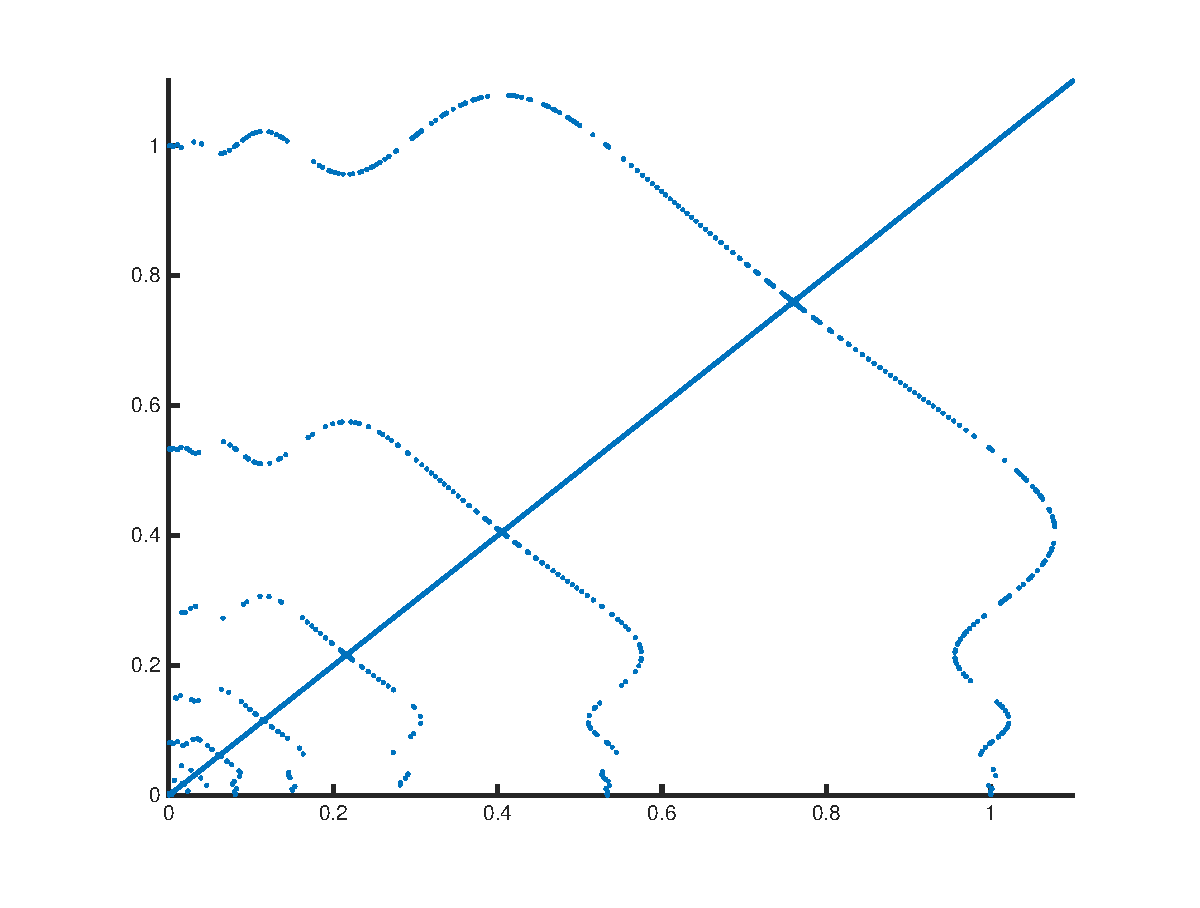
\includegraphics[width=10cm]{periodic/zeroset5}
\caption[Zero set of $H$]{Zero set of $H(a_0, a_1)$ for $\rho = 5$.}
\end{center}
\label{fig:Fzeronumeric}
\end{figure} 

In the next lemma, we will prove that pitchfork bifurcations occur on the diagonal in the zero set of $H(b_0, b_1)$ and identify their locations.

% lemma: pitchforks
\begin{lemma}\label{pitchforkH}
A discrete family of pitchfork bifurcations occurs along the diagonal in the zero set of $H(b_0, b_1)$ at 
\begin{align*}
(b_0, b_1) &= (b_k^*, b_k^*) && k \in \Z
\end{align*}
where 
\begin{equation}\label{pkstar}
b^*_k = e^{-\frac{1}{\rho} (k \pi + p^*) }
\end{equation}
and 
\begin{equation}\label{pstar}
p^* = \arctan \rho.
\end{equation}
Locally, the arms of the pitchfork bifurcations open upwards along the diagonal.
\begin{proof}
The proof is a straightforward, but tedious computation. Let $b^* = e^{-\frac{1}{\rho} p^*}$. First, we determine the locations of the pitchfork bifurcations along the diagonal. A necessary condition for these to occur is that the first derivative vanishes. The partial derivative of $H$ with respect to $b_0$ is
\begin{align*}
H_{b_0}(b_0, b_1) &= 
\sin \left( -\rho \log b_0 \right)
+ b_0 \cos \left( - \rho \log b_0 \right)- \rho \frac{1}{b_0} \\
&= \sin \left( - \rho \log b_0 \right) - \rho \cos \left( - \rho \log b_0 \right)
\end{align*}
Note that this does not depend on $b_1$. $H_{b_0}(b_0, b_1) = 0$ if and only if
\begin{align*}
\tan \left( -\rho \log b_0 \right) &=  \rho \\
-\rho \log b_0 &= \arctan \left( \rho\right) + k \pi && k \in \Z \\ 
b_0 &= \exp \left( -\frac{1}{\rho} \arctan \rho - \frac{k \pi}{\rho} \right) \\
&= \exp \left( -\frac{1}{\rho} \arctan \rho - \frac{k \pi}{\rho} \right)  \\
&= \exp \left( -\frac{1}{\rho} (k + \arctan \rho) \right) \\
&= b_k^*
\end{align*}

Next, we change coordinates so that the pitchfork bifurcation will occur along the $x$-axis. Let
\begin{align*}
x &= \frac{1}{2}(b_1 - b_0) \\
y &= \frac{1}{2}(b_1 + b_0)
\end{align*}
In terms of $b_0$ and $b_1$,
\begin{align*}
b_0 &= y - x \\
b_1 &= y + x
\end{align*}
Substituting these into $H(b_0, b_1)$ yields
\begin{equation}\label{Hxy}
H(x, y) = 
(y - x) \sin \left( -\rho \log(y - x) \right) - (y + x) \sin \left( - \rho \log (y + x) \right)
\end{equation}
Since $H(-x, y) = -H(x, y)$, $H(x,y)$ has the required symmetry for a pitchfork bifurcation; $y$ will be the bifurcation parameter. Fix $k \in \Z$. We will prove that in the $(x,y)$ coordinate system, a pitchfork bifurcation occur at $(x_0, y_0) = \left(0, b^*_k \right)$.

To show this, we evaluate a series of partial derivatives at $(x_0, y_0)$. For the first derivatives,
\begin{align*}
H_x(x, y) &= -\sin \left( - \rho \log(y - x) \right) - 
\sin \left( - \rho \log(y + x) \right)
+\rho \cos \left( - \rho \log(y - x) \right) + \rho \cos \left( - \rho \log(y + x) \right) \\
H_y(x, y) &= \sin \left( - \rho \log(y - x) \right) - 
\sin \left( - \rho \log(y + x) \right)
-\rho \cos \left( - \rho \log(y - x) \right) + \rho \cos \left( - \rho \log(y + x) \right)
\end{align*}
Plugging in $(x_0, y_0)$ and noting that $\sin(\arctan \rho) = \rho / \sqrt{1 + \rho^2}$ and $\cos(\arctan \rho) = 1 / \sqrt{1 + \rho^2}$, both $H_x(x_0, y_0) = 0$ and $H_y(x_0, y_0) = 0$. Next, we look at the second partial derivatives. For $H_{xx}$,
\begin{align*}
H_{xx}(x, y) &= 
-(y-x) \left(-\frac{\rho^2 \sin \left(\rho \log (y-x)\right)}{(y-x)^2}-\frac{\rho
   \cos \left(\rho \log (y-x) \right)}{(y-x)^2}\right)\\
   &+(x+y) \left(-\frac{\rho^2
   \sin \left(\rho \log (x+y)\right)}{(x+y)^2}-\frac{\rho \cos \left( \rho
   \log (x+y)\right)}{(x+y)^2}\right)\\
   &-\frac{2 \rho \cos \left(\rho \log
   (y-x) \right)}{(y-x)}+\frac{2 \rho \cos \left( \rho \log (x+y) \right)}{
   (x+y)}
\end{align*}
A tedious calculation, which can be verified by Mathematica, shows that $H_{xx}(x_0, y_0) = 0$. By symmetry, we also have $H_{yy}(x_0, y_0) = 0$. The mixed derivative $H_{xy}$ is
\begin{align*}
H_{xy}(x, y) &= -\frac{\rho^2 \sin \left(\rho \log (y-x)\right)}{(y-x)}-\frac{\rho^2 \sin
   \left(\rho \log (x+y)\right)}{(x+y)}+\frac{\rho \cos \left(\rho \log (y-x)\right)}{(y-x)}+\frac{\rho \cos \left( \rho \log (x+y) \right)}{(x+y)}
\end{align*}
Evaluating this at $(x_0, y_0)$, we have
\begin{align*}
H_{xy}(x_0, y_0) &= \frac{2 \rho}{b^*_k}\left( -\rho \sin \left(\rho \log b^*_k \right) + \cos \left(\rho \log b^*_k \right) \right)\\
&= \frac{2 \rho}{b^*_k}\left( -\rho \sin \left(\rho \log b^* + k \pi \right) + \cos \left(\rho \log b^* + k \pi \right) \right) \\
&= \frac{2 \rho}{b^*_k} (-1)^k \left( \rho \sin \left(\arctan \rho \right) + \cos \left(\arctan \rho \right) \right)\\ 
&= \frac{2 \rho}{p_n^*} (-1)^k \frac{\rho^2 + 1}{\sqrt{1 + \rho^2}} \\
&= (-1)^k 2 \rho \sqrt{1 + \rho^2} \: \exp{\left(\frac{1}{\rho} (\arctan \rho - k \pi) \right)}
\end{align*}
Since $\rho > 0$, this is nonzero. Let $c_1^k = H_{xy}(x_0, y_0)$. Finally, we check the third partial derivative with respect to $x$. This is another tedious calculation, but with the help of Mathematica we obtain
\begin{align*}
H_{xxx}(x_0, y_0)
&= -(-1)^k 2 \rho \sqrt{1 + \rho^2} \: \exp{\left(\frac{2}{\rho} (\arctan \rho - k \pi) \right)}
\end{align*}
Since $\rho > 0$, this is also nonzero. Let $c_2^k = -H_{xxx}(0, b^*_k)$.

We have verified that a pitchfork bifurcation occurs at $(0, b^*_k)$ for all $k \in \Z$. Near the bifurcation points $(0, b_k^*)$, we have the Taylor expansions
\begin{align*}
H(x, y) &= c_1^k x (y - b_k^*) - \frac{c_2^k}{6} x^3 + \mathcal{O}(x^4) \\
&= c_1^k x \left( (y - b_k^*) - \frac{c_2^k}{6 c_1^k } x^2 \right) + \mathcal{O}(x^4) \\
&= c_1^k x \left( (y - b_k^*) - \frac{c_3^k}{6} x^2 \right) + \mathcal{O}(x^4) \\
\end{align*}
where
\begin{equation*}
c_3^k = \exp{\left(\frac{1}{\rho} (\arctan \rho - k \pi) \right)} > 0
\end{equation*}
To leading order, the arms of the pitchforks are upwards-opening parabolas of the form 
\begin{align*}
y &= b_k^* + \frac{c_3^k}{6} x^2
\end{align*}
Since the above change of coordinates is a rotation by $\pi/4$, we conclude that pitchfork bifurcations occur in the original $(b_0, b_1)$ coordinate system at $(b_0, b_1) = (b_k^*, b_k^*)$. The arms of the pitchforks are, to leading order, parabolas which open upwards along the diagonal.
\end{proof}
\end{lemma}

\section{Parameterization of zero set of $H$}

Now that we have located the pitchfork bifurcations, we will devise a natural parameterization for the zero set of $H(b_0, b_1)$. Since the zero set is symmetric across the diagonal we only need to consider the case where $b_0 \geq b_1$. The parameterization works as follows. Choose any two nonnegative integers $m_1 \geq m_0$. Then the point
\[
(b_0, b_1) = \left( e^{\frac{-m_0 \pi}{\rho}}, e^{\frac{-m_1 \pi}{\rho}}\right)
\]
is in the zero set of $H$. We will use these points to ``anchor'' our parameterization. We will then use a phase parameter $\theta$ to connect these anchor points. We define our parameterization in the next lemma.

% lemma : parameterization of zero set of H

\begin{lemma}\label{thetaparamlemma}
For every choice of nonnegative integers $m_0$ and $m_1$ with $m_1 \geq m_0$, there is a smooth family of solutions
\[
\left( b_0( m_0, m_1, \theta), b_1( m_0, m_1, \theta) \right)
\]
to $H(b_0, b_1) = 0$, where $\theta \in I = [-\pi + p^*, p^*]$. The parameterization is given explicity by
\begin{equation}\label{thetaparam}
\begin{aligned}
b_0( m_0, m_1, \theta) &= \exp\left[ -\frac{1}{\rho}(m_0 \pi + \theta^*(\theta, m_1 - m_0) \right] \\
b_1( m_0, m_1, \theta) &= \exp\left[ -\frac{1}{\rho}(m_1 \pi + \theta) \right]
\end{aligned}
\end{equation}
where for all nonnegative integers $m$, $\theta^*(\theta, m) : I \rightarrow \R$ is smooth in $\theta$ and has the following properties.
\begin{enumerate}[(i)]
\item $\theta^*(0; m) = 0 \text{ for all } m$
\item $|\theta^*(\theta; m)| \leq |\theta|$
\item $|\theta^*(\theta; m)| \leq C \exp\left(-\frac{m \pi}{\rho} \right)$
\item $\theta^*(\theta; 0) = \theta $
\item $\theta^*(p^*; m) = \theta^*(-\pi+p^*; m+1)$
\end{enumerate}
In particular, $\theta^*(p^*, 0) = \theta^*(\pi - p^*, 1) = p^*$.
\begin{proof}
The proof is essentially routine computation. We start with the ansatz
\begin{equation}\label{thetaansatz}
\begin{aligned}
b_0( m_0, m_1, \theta) &= \exp\left[ -\frac{1}{\rho}(m_0 \pi + \theta^*) \right] \\
b_1( m_0, m_1, \theta) &= \exp\left[ -\frac{1}{\rho}(m_1 \pi + \theta) \right]
\end{aligned}
\end{equation}
Our goal is to solve for $\theta^*$ in terms of $\theta$. We proceed in the following steps.
\begin{enumerate}

\item First, we show that $\theta^*$ only depends on the difference $m_1 - m_0$. Substituting the ansatz \cref{thetaansatz} into $H(b_0, b_1) = 0$, we have
\begin{align*}
0 &= e^{-\frac{1}{\rho}m_0 \pi}e^{-\frac{1}{\rho}\theta^*}\sin(m_0 \pi + \theta^*) - e^{-\frac{1}{\rho}m_1 \pi}e^{-\frac{1}{\rho}\theta}\sin(m_1 \pi + \theta) \\
&= e^{-\frac{1}{\rho}m_0 \pi} \left( e^{-\frac{1}{\rho}\theta^*}(-1)^{m_0} \sin \theta^* - e^{-\frac{1}{\rho}(m_1 - m_0) \pi} (-1)^{m_0} (-1)^{m_1 - m_0} e^{-\frac{1}{\rho}\theta}\sin \theta \right) \\
&= e^{-\frac{1}{\rho}m_0 \pi} (-1)^{m_0} \left( e^{-\frac{1}{\rho}\theta^*}\sin \theta^* - e^{-\frac{1}{\rho}(m_1 - m_0) \pi} (-1)^{m_1 - m_0} e^{-\frac{1}{\rho}\theta}\sin \theta \right) 
\end{align*}
Dividing by $e^{-\frac{1}{\rho}m_0 \pi} (-1)^{m_0}$, we wish to solve
\begin{equation}\label{thetaeq1}
e^{-\frac{1}{\rho}\theta^*}\sin \theta^* = e^{-\frac{1}{\rho}(m_1 - m_0) \pi} (-1)^{m_1 - m_0} e^{-\frac{1}{\rho}\theta}\sin \theta 
\end{equation}
Since the RHS only depends on the difference $m_1 - m_0$, let $m = m_1 - m_0$. Then it suffices to find a solution $\theta^*(\theta, m)$ to 
\begin{equation}\label{thetaeq2}
g(\theta^*) = t(m) g(\theta)
\end{equation}
for all nonnegative integers $m$, where
\begin{align*}
g(\theta) &= e^{-\frac{1}{\rho}\theta}\sin \theta  \\
t(m) &= e^{-\frac{1}{\rho}m \pi} (-1)^m
\end{align*}

\item For $m = 0$, $t(0) = 1$, thus $\theta^*(\theta, 0) = \theta$.

\item Now consider $m \geq 1$. We start by characterizing the function $g(\theta)$, which we do in the following steps.
\begin{enumerate}
	\item First, we show that $g(\theta)$ is strictly increasing on $I$. The derivative of $g$ is 
	\begin{equation}\label{gprime}
	g'(\theta) = e^{ -\frac{1}{\rho} \theta } \left( \cos \theta - \frac{1}{\rho} \sin \theta \right)
	\end{equation}
	At the right endpoint of $I$,
	\begin{align*}
	g'(p^*) &= g'(\arctan \rho) \\
	 &= e^{ -\frac{1}{\rho} \arctan \rho } \left(\cos(\arctan \rho) - \frac{1}{\rho} \sin(\arctan \rho)\right) \\
	&= e^{ -\frac{1}{\rho} \arctan \rho } \left(\frac{1}{\sqrt{1 + \rho^2}} - \frac{1}{\rho} \frac{\rho}{\sqrt{1 + \rho^2}}\right) = 0
	\end{align*}
	Similarly, at the right endpoint $I$, $g'(\pi - P^*) = 0$. 

	The only critical point of $g'(\theta)$ on $I_\rho$ is a local maximum at $\theta = - \pi + 2 p^*$. Since $g'(\theta) > 0$ on the interior of $I$ and is zero at the endpoints, $g(\theta)$ is strictly increasing on $I$. Furthermore, we can easily show that the only zero of $g(\theta)$ on $I$ is at $\theta = 0$.
	
	\item Since $g$ is strictly increasing on $I$, it is invertible on $g(I)$. Evaluating $g$ at the endpoints of $I$, let
	\begin{equation}\label{grange}
	I^{-1} = g(I) = [-e^{\frac{1}{\rho}\pi} T, T]
	\end{equation}
	where 
	\begin{equation}\label{defT}
	T = e^{-\frac{1}{\rho}p^*} \sin p^* = \frac{\rho}{\sqrt{1+\rho^2}}e^{-\frac{1}{\rho}\arctan \rho}
	\end{equation}
	Thus $g: I \rightarrow I^{-1}$ is a bijection, and $g^{-1}: I^{-1} \rightarrow I$ is also strictly increasing. Since $g(0) = 0$, $g^{-1}(0) = 0$ as well.
\end{enumerate}

\item We can now solve $g(\theta^*) = t(m) g(\theta)$ for $m \geq 1$. Using \cref{grange}, for all $\theta \in I$,
	\begin{equation}\label{RHSbounds}
	t(m)g(\theta) \in
	\begin{cases}
	[-e^{-\frac{1}{\rho}(m-1) \pi} T, e^{-\frac{1}{\rho}m \pi} T] & m \text{ even }\\
	[-e^{-\frac{1}{\rho}m \pi} T, e^{-\frac{1}{\rho}(m-1) \pi} T] & m \text{ odd }
	\end{cases}
	\end{equation}
	In both cases, since $m \geq 1$, the RHS of \cref{RHSbounds} is contained in $I^{-1}$, thus we can solve for $\theta^*$. For $m \geq 1$, define
	\begin{equation}\label{solvethetastar}
	\theta^*(\theta, m) = g^{-1}\left( t(m) g(\theta) \right)
	\end{equation}
	Since $g(0) = 0$, it follows that $\theta^*(0, m) = 0$ for all $m$.	Since for all $m \geq 0$, $\theta^*(\theta, m) \in I_\rho$, the parameterizations for different $m$ can only overlap at the endpoints of $I$.

\item Next, we show that $|\theta^*(\theta, m)| \leq |\theta|$. For $m = 0$, we have equality. If $m = 1$ and $\theta = -\pi + p^*$,
\begin{align*}
t(-\pi + p^*)g(-\pi + p^*) &= -e^{-\frac{1}{\rho}\pi}e^{-\frac{1}{\rho}(-\pi+p^*)}\sin(-\pi + p^*) \\
&= e^{-\frac{1}{\rho}p^*} \sin p^* = T,
\end{align*}
thus $\theta^*(-\pi + p^*, 1) = -\pi + p^*$. For any other $m$ and $\theta$, it follows from \cref{RHSbounds} that $t(m)g(\theta) \in [e^{-\frac{1}{\rho}\pi}T, T)$, which is strictly contained in $I^{-1}$. Since $g^{-1}$ is strictly increasing and $g(0) = 0$, we conclude that $|\theta^*(\theta, m) \leq |\theta|$.

\item Next, we show that the parameterizations match up at the endpoints. For $m \geq 0$, we evaluate
\begin{align*}
\theta^*(p^*, m) &= g^{-1}\left( e^{-\frac{1}{\rho}m \pi} (-1)^m e^{-\frac{1}{\rho}p^*} \sin p^* \right)
\end{align*}
and
\begin{align*}
\theta^*(-\pi + p^*, m+1) &= g^{-1}\left( e^{-\frac{1}{\rho}(m+1) \pi} (-1)^{m+1} e^{-\frac{1}{\rho}(-\pi + p^*)} \sin (-\pi + p^*) \right) \\
&=g^{-1}\left( e^{-\frac{1}{\rho}m \pi} (-1)^m e^{-\frac{1}{\rho}p^*} \sin p^* \right)
\end{align*}
By uniqueness of the inverse $g^{-1}$, these must be equal. In particular, 
\[
\theta^*(p^*, 0) = \theta^*(\pi - p^*, 1) = p^*
\]

\item Finally, we obtain a bound on $\theta^*(\theta, m)$. For $m \geq 2$ and all $\theta \in I$, $t(m)g(\theta) \in \tilde{I}$, which is strictly contained in $I$. Since $g'(0) = 0$ only at the endpoints of $I$ and is positive in the interior of $I$, $g'(\theta)$ is bounded below by a constant $L$ on $\tilde{I}$. Thus for all $m \geq 2$ and all $\theta \in I$, $[g^{-1}]'(\theta) \leq 1/L$. It follows from \cref{RHSbounds} that 
\[
|t(m)g(\theta)| \leq e^{-\frac{1}{\rho}(m - 1)\pi}T
\]
Combining these, since $g(0) = 0$, we have for $m \geq 2$ and all $\theta \in I$, 
\begin{align*}
|\theta^*(\theta, m)| \leq \frac{1}{L}e^{-\frac{1}{\rho}(m - 1)\pi}T
\end{align*}
Since the constants out front do not matter and $|\theta^*(\theta, m)| \leq |\theta|$ for all $m$, we can find a constant $C$ such that for all $m \geq 0$ and all $\theta \in I$,
\begin{align*}
|\theta^*(\theta, m)| \leq C e^{-\frac{1}{\rho} m \pi}
\end{align*}
This bound is uniform in $\theta$.
\end{enumerate}

\end{proof}
\end{lemma}

Now that we have our parameterization for $r = 0$, we would like to use it to solve \eqref{Geq} for small $r$. When we perturb $r$ away from 0, we will generically lose the pitchfork bifurcation structure. In addition, since this relies on the implicit function theorem, we will not be able to use the implicit function theorem at the pitchfork bifurcation points. In the next section, we prove the existence theorem for periodic multi-pulses. After that, we will show that in the special case of the periodic 2-pulse, the entire bifurcation structure of $H$ persists for sufficiently small $r$.

\section{Proof of Theorem \ref{perexist}}

By Lemma \ref{diagonalG}, a periodic $n-$pulse exists if and only if the $n-1$ jump conditions
\begin{align}\label{Geq2}
G_j(b_0, \dots, b_{n-1}, r) = b_j \sin \left( -\rho \log b_j \right) - b_{n-1} \sin \left( -\rho \log b_{n-1} \right) + \mathcal{O}(r^{\gamma / 2 \alpha}) &= 0 && j = 0, \dots, n-2
\end{align}
are satisfied. For $r = 0$, $G_j(b_0, \dots, b_{n-1}, 0) = H(b_j, b_{n-1})$ for each $j$. Since each equation is of the same form, with $b_{n-1}$ appearing in all of them, we can parameterize our solution using \cref{thetaparamlemma}. First, we make the following definition.

\begin{definition}
For $n \geq 2$, a \emph{periodic parameterization} of a periodic $n$-pulse is a sequence of parameters $(m_0, \dots, m_{n-1}, \theta)$, where
\begin{enumerate}[(i)]
\item $m_j$ is a nonnegative integer with
\begin{enumerate}
\item at least one of the $m_j \in \{0, 1\}$.
\item $m_{n-1} \geq m_j$ for $j = 0, \dots, n-2$.
\end{enumerate}
\item $\theta \in (-\pi + p^*, p^*]$.
\end{enumerate}
\end{definition}
The selection of $m_{n-1}$ as the largest of the $m_j$ is made for notational convenience and to allow the parameterization to be unique. Using Lemma \ref{thetaparamlemma}, let
\begin{equation}\label{thetaparammulti}
\begin{aligned}
b_j( m_j, m_{n-1}, \theta) &= \exp\left[ -\frac{1}{\rho}(m_j \pi + \theta^*(\theta, m_{n-1} - m_j) \right] && j = 0, \dots, n-2 \\
b_{n-1}( m_{n-1}, \theta) &= \exp\left[ -\frac{1}{\rho}(m_{n-1} \pi + \theta) \right]
\end{aligned}
\end{equation}
From Lemma \ref{thetaparamlemma},
\begin{align*}
H(b_j( m_j, m_{n-1}, \theta), b_{n-1}( m_{n-1}, \theta) ) &= 0 && j = 0, \dots, n-2
\end{align*}
Let
\[
b^* = (b_0( m_0, m_{n-1}, \theta), \dots, b_{n-2}( m_{n-2}, m_{n-1}, \theta) ) \in \R^{n-1}
\]
Substituting $b_{n-1}(m_{n-1}, \theta)$ for $b_{n-1}$ in \eqref{Geq2}, define $G: \R^{n-1} \times \mathcal{R} \rightarrow \R^{n-1}$ by $G = (G_0, \dots, G_{n-2})^T$, where 
\begin{equation*}
G_j(b, r) = b_j \sin \left( -\rho \log b_j \right) - b_{n-1}(m_{n-1}, \theta) \sin \left( -\rho \log b_{n-1}(m_{n-1}, \theta) \right) + \mathcal{O}(r^{\gamma / 2 \alpha})
\end{equation*}
and $b = (b_0, \dots, b_{n-1})$. From our definition of $b^*$, $G(b^*, 0) = 0$.

Next, we evaluate the partial derivatives of $G_k$ with respect to $b_j$. For $j \neq k$, 
\[
\partial_{b_j} G_k(b, r) = \mathcal{O}(r^{\gamma/2\alpha})
\]
where the order of the remainder term comes from Lemma \ref{jumplemma3}. For $j = k$, 
\begin{align*}
\partial_{b_j} G_j(b, r) &= 
\sin \left( -\rho \log b_j \right) - \rho b_j \cos \left( -\rho \log b_j \right) \frac{1}{b_j} + \mathcal{O}(r^{\gamma/2\alpha}) \\
&= \sin \left( -\rho \log b_j \right) - \rho \cos \left( -\rho \log b_j \right) + \mathcal{O}(r^{\gamma/2\alpha}) 
\end{align*}
Evaluating these at $r = 0$ and $b = b^*$, the Jacobian matrix $D_b G(b^*,0)$ is diagonal, with diagonal entries given by 
\begin{align*}
\partial_{b_j} G_j(b^*, 0)
&= \sin \left( -\rho \log b_j(m_j, \theta) \right) - \rho \cos \left( -\rho \log b_j(m_j, \theta) \right)
\end{align*}

We can use the implicit function theorem as long these partial derivatives are all nonzero. From Lemma \ref{pitchforkH}, $\partial_{b_j} G_j(b, 0) = 0$ if and only if $b_j = b_k^*$, where $b_k^*$ is one of the pitchfork bifurcation points in the zero set of $H$. To avoid this, by Lemma \ref{thetaparamlemma}, it suffices to exclude $\theta \in \{ -\pi + p^*, p^* \}$, which we do in the statement of the theorem.

Thus, for sufficiently small $r$, we can use the implicit function theorem to solve for $b$ in terms of $r$ near $b^*$. Specifically, there exists $r_* > 0$ and a smooth function $b: \mathcal{R} \cap [0, r_*] \rightarrow \R^{n-1}$ such that $b(0) = b^*$ and $G(b(r),r) = 0$. Write $b$ in terms of its component functions as
\[
b(r) = \left( b_0(r), \dots, b_{n-2}(r) \right)
\]
Using \cref{Xjscale}, for $j = 0, \dots, n-2$, the pulse distances $X_j$ are given by
\begin{align*}
X_j &= -\frac{1}{2\alpha}\log(b_j(r) r) - \frac{\phi}{2 \beta} \\
&= \frac{1}{2\alpha}|\log r| + \frac{1}{2\beta}\big[ -\rho \log(b(r)) \big] + L_0
\end{align*}
where we define $L_0 = \frac{\phi}{2 \beta}$. For $j = 0, \dots, n-2$, define $t_j(r; m_j, \theta): \mathcal{R} \rightarrow \R$ by
\begin{equation}\label{deftj}
t_j(r; m_j, m_{n-1}, \theta) = -\rho \log b_j(r)
\end{equation}
The functions $t_j(r; m_j, m_{n-1}, \theta)$ are smooth in $r$, and from \cref{thetaparammulti}, 
\[
b_j(0) = \exp\left[ -\frac{1}{\rho}(m_j \pi + \theta^*(\theta, m_{n-1} - m_j) \right]
\]
\begin{align*}
t_j(0; m_j, m_{n-1}, \theta) &= m_j \pi + \theta^*(\theta, m_{n-1} - m_j)
\end{align*}
Using \cref{thetaparammulti} again, the final pulse length $X_{n-1}$ is given by 
\begin{align*}
X_{n-1}(r; m_{n-1}, \theta) &= \frac{1}{2 \alpha_0} |\log r| + \frac{1}{2 \beta_0}\big( (2 m + m_{n-1})\pi + \theta \big) + L_0
\end{align*}
The domain length $X$ is obtained by adding up the $X_j$.

\section{Periodic 2-pulse}

For the periodic 2-pulse, we will be able to provide the complete bifurcation structure. In this case, we only have to solve the single jump equation
\begin{equation}\label{2pulsedefG}
G(b_0, b_1, r) = b_0 \sin \left( -\rho \log b_0 \right) - b_1 \sin \left( -\rho \log b_1 \right) + \mathcal{O}(r^{\gamma / 2 \alpha}) = 0 \\
\end{equation}

First, we will show that that the pitchfork bifurcation persists for small $r$. In the first lemma, we show that $G$ has the same symmetries as $H$.

% lemma : symmetries of G
\begin{lemma}\label{Gsymm}
For sufficiently small $r$, we have the symmetry relation
\begin{equation}\label{Gsymmjump1}
G(b_0, b_1, r) = -G(b_1, b_0, r)
\end{equation}
In particular, 
\[
G(b_0, b_0, r) = 0
\]
\begin{proof}
In Lemma \ref{solvewithjumps}, we showed that given an ordered pair of pulse distances $(X_0, X_1)$, as long as the $X_i$ are sufficiently large, there exists a unique piecewise solution $\{ U_0^-(x), U_0^+(x), U_1^-(x), U_1^+(x) \}$ to \eqref{systemwithjumpZ} which generically has two jumps at $x = 0$ in the direction of $\Psi(0)$. These jumps are functions of $X_0$ and $X_1$ and are given by
\begin{equation}\label{xijumps}
\begin{aligned}
\xi_0(X_0, X_1) &= \langle \Psi(0), U_0^+(0) - U_0^-(0) \rangle  \\
\xi_1(X_0, X_1) &= \langle \Psi(0), U_1^+(0) - U_1^-(0) \rangle 
\end{aligned}
\end{equation}

For a given ordered pair of lengths $(X_0, X_1)$, let $\{ U_0^-(x), U_0^+(x), U_1^-(x), U_1^+(x) \}$, pieced together from left to right, be the unique solution to \eqref{systemwithjumpZ}. If swap $X_0$ and $X_1$ to get the ordered pair $(X_1, X_0)$, we have another solution to \eqref{systemwithjumpZ}; by uniqueness, this solution must be given by $\{ U_1^-(x), U_1^+(x), U_0^-(x), U_0^+(x)\}$ since we are on a periodic domain. Thus for the jumps $\xi_j$ we have
\begin{equation}\label{xiswapX}
\begin{aligned}
\xi_0(X_1, X_0) &= \langle \Psi(0), U_1^+(0) - U_1^-(0) \rangle = \xi_1(X_0, X_1) \\
\xi_1(X_1, X_0) &= \langle \Psi(0), U_0^+(0) - U_0^-(0) \rangle = \xi_0(X_0, X_1)
\end{aligned}
\end{equation}

If we keep the ordered pair $(X_0, X_1)$ but replace $x$ with $-x$, $\{ U_1^+(-x), U_1^-(-x), U_0^+(-x), U_0^-(-x)\}$, pieced together from left to right, also satisfies \eqref{systemwithjumpZ}. By uniqueness, $U_1^+(0) = U_0^-(0)$ and $U_1^-(0) = U_0^+(0)$. Thus for the jump $\xi_0$, we have
\begin{align*}
\xi_0(X_0, X_1) &= \langle \Psi(0), U_0^+(0) - U_0^-(0) \rangle \\
&= \langle \Psi(0), U_1^-(0) - U_1^+(0) \rangle \\
&= -\langle \Psi(0), U_1^+(0) - U_1^-(0) \rangle \\
&= -\xi_1(X_0, X_1) \\
&= -\xi_0(X_1, X_0)
\end{align*}
where for the last equality we used \eqref{xiswapX}. Similarly, $\xi_1(X_0, X_1) = -\xi_0(X_1, X_0)$. The result follows since swapping $X_0$ and $X_1$ in $\xi(X_0, X_1)$ is equivalent to swapping $b_0$ and $b_1$ in \cref{Gsymmjump1}.

\end{proof}
\end{lemma}

In the next lemma, we show that the pitchfork bifurcations persists on the diagonal for sufficiently small $r$. Since for a periodic parameterization of a periodic 2-pulse we require $m_0 \in \{0, 1\}$, we only have to show this result for two pitchfork bifurcations.

% lemma :Persistence of pitchfork

\begin{lemma}\label{pitchpersist}
There exists $r_2 > 0$ such that for $m_0 \in \{0, 1\}$ and $r \leq r_2$, there is a non-degenerate pitchfork bifurcation in the zero set of $G(b_0, b_1, r)$ at $(b_{m_0}^*(r),b_{m_0}^*(r))$, and 
\begin{equation*}
b_{m_0}^*(r) \rightarrow b_{m_0}^* \text{ as } r \rightarrow 0
\end{equation*}
\begin{proof}
For simplicity, take $m_0 = 0$. The proof is identical for $m_0 =1$. In Lemma \ref{pitchforkH}, we showed that a pitchfork bifurcation occurs in the zero set of $H(b_0, b_1)$ at $(b_0^*, b_0^*)$. As in Lemma \ref{pitchforkH}, we make the change of coordinates $(b_0, b_1) \mapsto (x, y)$, so that $(0, b_0^*)$ is a pitchfork bifurcation point of $G(x, y, 0)$. By Lemma \ref{Gsymm}, we have the symmetry 
\[
G(-x, y, r) = -G(x, y, r)
\]
in this coordinate system, which is the required symmetry for a pitchfork bifurcation to occur. In addition, this implies that $G(0, y, r) = 0$ for all $y$. We now prove the existence of a pitchfork bifurcation along this line. While this is a standard result from bifurcation theory, we present the proof below for completeness. 

Since a necessary condition for a pitchfork to occur is $G_x(x, y, r) = 0$, we will look at the system
\begin{equation*}
K(x,y,r) = (G(x,y,r), G_x(x,y,r)) = 0
\end{equation*}
From Lemma \ref{pitchforkH}, $G_x(0,b_0^*,0) = G_y(0, n_0^*, 0) = 0$, so $D_{x,y}K(0,b_0^*,0)$ is singular. Since we cannot apply the implicit function theorem at $(0, b_0^*)$, we will do a Lyapunov-Schmidt reduction. In Lemma \ref{pitchforkH}, we showed that $G_{xy}(0, b_0^*, 0) = 2 \rho/b_0^* \sqrt{1 + \rho^2} \neq 0$. Thus we can use the implicit function theorem to solve $K_2(x,y,r) = G_x(x,y,r) = 0$ for $y$ in terms of $x$ and $r$ near $(x,y,r) = (0, b_0^*, 0)$. Specifically, there exists $r_2 > 0$, an open interval $(-a, a)$, and a unique smooth function $y = y^*(x, r)$ such that $y^*(0, 0) = b_0^*$ and $G_x(x, y^*(x, r), r) = 0$ for all $x \in (-a, a)$ and $r < r_2$.

Take $y = y^*(x, r)$ in the equation for $G$. We will now solve
\begin{equation*}
G(x, y^*(x, r), r) = 0,
\end{equation*}
which always has a solution when $x = 0$. We will show that a pitchfork bifurcation occurs at $(0, y^*(0, r), r)$ by verifying the conditions needed for this bifurcation to occur. First, since $G(x, y, r)$ is an odd function in $x$, $G_y(0, y, r) = 0$ and $G_{xx}(0, y, r) = 0$ for all $x, r$. It follows that $G_y(0, y^*(0, r), r) = 0$ and $G_{xx}(0, y^*(0, r), r) = 0$.

All that remains is to show that $G_{xy}$ and $G_{xxx}$ are nonzero at $(0, y^*(0, r), r)$. From Lemma \ref{pitchforkH}, $G_{xy}(0, b_0^*, 0) = c_1^0 \neq 0$. Since $G_{xy}$ and $y^*$ are smooth, $G_{xy}(0, y^*(0, r), r) \rightarrow c_1^0 \text{ as } r \rightarrow 0$. Thus, reducing $r_2$ if necessary, $G_{xy}(0, y^*(0, r), r) \neq 0$ for all $r < r_2$. Similarly, from Lemma \ref{pitchforkH}, $G_{xxx}(0, p^*) = c_2^0 \neq 0$. By the same argument, we conclude that $G_{xxx}(0, y^*(0, r), r) \neq 0$ for $r < r_2$.

Let $b_0^*(r) = y^*(0, r)$. Changing back to the original $(b_0, b_1)$ coordinates, there is a pitchfork bifurcation at $(b_0^*(r), b_0^*(r))$, and $b_0^*(r) \rightarrow b_0^*$ as $r \rightarrow 0$.
\end{proof} 
\end{lemma}

In Lemma \ref{Gsymm}, we showed that for sufficiently small $r$, $G(b_0, b_0, r) = 0$, so the zero set of $G$ contains the diagonal. In the next lemma, we show that the arms of the pitchfork also persist for sufficiently small $r$. As in the previous lemma, we only need to consider two pitchforks corresponding to $m_0 = 0$ and $m_0 = 1$. By symmetry, we also only need to show it for the lower arm. 

\begin{lemma}\label{armpersists}
Choose any $\delta > 0$. Then there exists $r_3 > 0$ such that for $m_0 \in \{0, 1\}$ and $r \leq r_3$, the portion of the zero set of $G(b_0, b_1, r)$ corresponding to lower arm of the pitchfork at $(b_{m_0}^*(r), b_{m_0}^*(r))$ is parameterized by
\begin{align*}
(b_0, b_1) = (\tilde{b}_0(s; m_0, r), \tilde{b}_1(s)) && s \in [p^* + \delta, \infty)
\end{align*}
where
\begin{align}\label{tildeb1}
\tilde{b}_1(s) &= e^{-\frac{1}{\rho}s} 
\end{align}

\begin{proof}
For simplicity, take $m_0 = 0$. The proof is identical for $m_0 = 1$. For every positive integer $m_1$ with $m_1 \geq 1$, using the parameterization in Lemma \ref{thetaparamlemma}, let
\begin{equation}\label{thetaparam}
\begin{aligned}
b_0( m_1, \theta) &= \exp\left[ -\frac{1}{\rho}\theta^*(\theta, m_1 - m_0) \right] \\
b_1( m_1, \theta) &= \exp\left[ -\frac{1}{\rho}(m_1 \pi + \theta) \right]
\end{aligned}
\end{equation}
Since these families connect together at their endpoints, define $\tilde{b}_1(s)$ by \cref{tildeb1}. For any $s_1 > p^*$, let
\begin{equation}
\begin{aligned}
m(s) &= \lceil \frac{s - p^*}{\pi} \rceil \\
\theta(s) &= s - m(s) \pi
\end{aligned}
\end{equation}
Then we define $\tilde{b}_0(s)$ by
\begin{equation}\label{tildeb0}
\tilde{b}_0(s) = b_0(m(s), \theta(s)).
\end{equation}
Thus the continuous curve 
\begin{align*}
(b_0, b_1) &= (\tilde{b}_0(s), \tilde{b}_1(s)) && s > p^*
\end{align*}
parameterizes the lower arm of the pitchfork corresponding to $m_0 = 0$ when $r = 0$. We will show that this curve persists for small $r$. For $\delta > 0$, let $X$ be the Banach space
\[
X = C_b([p^* + \delta, \infty, \R)
\]
equipped with the uniform norm. For $b \in X$, define $\tilde{G}: X \times \mathcal{R} \rightarrow X$ by
\begin{align*}
[\tilde{G}(b, r)](s) &= G(b(s), \tilde{b}_1(s), r)
\end{align*}
Specifically, we have
\begin{align*}
[\tilde{G}(b, r)](s) &= b_0 \sin(-\log b_0) - e^{-\frac{1}{\rho}s} \sin s + \mathcal{O}(r^{\gamma/2\alpha}).
\end{align*}
Specifially, if $b(s)$ is bounded, so is $[\tilde{G}(b, r)](s)$. Next, we show that the Fr\'echet derivative of $\tilde{G}(b,r)$ with respect to $b$ at $(b, r) = (b, 0)$ is, as expected, the function 
\begin{equation}
f(s) = G_{b_0}(b(s), \tilde{b}_1(s), 0) 
\end{equation}
Using the definition of the Fr\'echet derivative, we need to show that
\begin{align}
\lim_{\|y\| \rightarrow 0} \frac{\| \tilde{G}(b + y, 0) - \tilde{G}(b, 0) - fy\|}{\|y\|} = 0
\end{align}
For $b(s) \in X$ and $s \in [p^* + \delta, \infty)$,
\begin{align*}
&\frac{ \left| [\tilde{G}(b + y, 0)](s) - [\tilde{G}(b, 0)](s) - f(s) y(s) \right| }{||y||} \\
&=\frac{ \left| G(b(s) + y(s), \tilde{b}_1(s), 0) - G(b(s), \tilde{b}_1(s), 0) - f(s) y(s) \right| }{\|y\|} \\
&\leq \frac{\left| G(b(s) + y(s), \tilde{b}_1(s), 0) - G(b(s), \tilde{b}_1(s), 0) - f(s) y(s)\right|}{|y(s)|} \frac{|y(s)|}{\|y\|} \\
&\leq \left| \frac{ G(b(s) + y(s), \tilde{b}_1(s), 0) - G(b(s), \tilde{b}_1(s), 0) - f(s) y(s)}{y(s)} \right| \\
&= \left| \frac{ G(b(s) + y(s), \tilde{b}_1(s), 0) - G(b(s), \tilde{b}_1(s), 0)}{y(s)} - G_{b}(b(s), \tilde{b}_1(s), 0) \right|
\end{align*}
Since we are taking $\|y\| \rightarrow 0$, $|y(s)| \rightarrow 0$ for each $s \in [p^* + \delta, \infty)$. Thus for each $s$, the RHS tends to 0 as $\|y\| \rightarrow 0$ by the definition of the partial derivative on $\R$. Since $G$ is smooth and both $b(s)$ and $\tilde{b}(s)$ are bounded, the RHS above is uniformly bounded in $s$. The result follows by taking the supremum over all $s \in [p^* + \delta, \infty)$.

By Lemma \ref{pitchforkH}, the derivative $G_{b_0}(b_0, b_1, 0) = H_{b_0}(b_0, b_1) = 0$ if and only if $(b_0, b_1)$ is one of the pitchfork bifurcation points. By construction and the parameterization in \cref{thetaparamlemma}, the curve $(\tilde{b}_0(s), \tilde{b}_1(s))$ only hits one of these points when $s = p^*$. 

Recall from the parameterization \cref{thetaparam} that 
\[
b_0( 0, m_1, \theta) = \exp\left[ -\frac{1}{\rho}\theta^*(\theta, m_1 - m_0) \right] \\
\]
If $\theta^*(\theta, m_1 - m_0) = 0$, then $G_{b_0}(b_0( 0, m_1, \theta), b_1( 0, m_1, \theta), 0) = -\rho$. By the bound on $\theta^*(\theta; m)$ from Lemma \ref{thetaparamlemma} and the continuity of $G_{b_0}(b_0, b_1, 0)$, there exists a positive integer $K$ such that for all $m_1 \geq K$,
\[
|G_{b_0}(b_0( 0, m_1, \theta), b_1( 0, m_1, \theta), 0)| \geq \frac{\rho}{2} 
\]
Thus by the definitions of $\tilde{b}_0(s)$ and $\tilde{b}_1(s)$, for all $s \geq K \pi$,
\[
|G_{b_0}(\tilde{b}_0(s), \tilde{b}_1(s), 0)| \geq \frac{\rho}{2} 
\]
Since the curve $(\tilde{b}_0(s), \tilde{b}_1(s)$ is continuous, $G_{b_0}(b_0, b_1, 0)$ is continuous,  and $G_{b_0}(\tilde{b}_0(s), \tilde{b}_1(s), 0) = 0$ only at the $s = p^*$, there exists $\eta = \eta(\delta)$ such that for $s \in [p^* + \delta, K \pi]$,
\[
|G_{b_0}(\tilde{b}_0(s), \tilde{b}_1(s), 0)| \geq \eta
\]
Combining these, for all $s \geq p^* + \delta$,
\begin{align*}
|G_{b_0}( \tilde{b}_0(s), \tilde{b}_1(s), 0)| \geq \min\{ \eta, \rho/2\}.  
\end{align*}
This implies that the Fr\'echet derivative $D_{b_0} \tilde{G}(\tilde{b}_0, 0)$ is invertible, and the inverse has bound
\[
[D_{b_0} \tilde{G}(\tilde{b}_0, 0)]^{-1} \leq \frac{1}{\min\{ \eta, \rho/2\}}
\]
Thus $D_{b_0} \tilde{G}(\tilde{b}_0, 0)$ is a Banach space isomorphism. Using the implit function theorem for Banach spaces, there exists $r_3 > 0$ and a unique smooth function $b: \mathcal{R} \rightarrow X$ with $b(0) = \tilde{b}_0$ such that for all $r \leq r_3$, $\tilde{G}(b(r), r) = 0$. Using the definition of $\tilde{G}$, for all $r \leq r_3$ and $s \in [p^* + \delta, \infty)$,
\begin{align*}
G([b(r)](s), \tilde{b}_1(s), r) = 0
\end{align*}
Taking $\tilde{b}_0(s; r) = [b(r)](s)$, the result follows.
\end{proof}
\end{lemma} 

In the final lemma, we show that for sufficiently small $r$, the lower arm of the pitchfork connects to the pitchfork bifurcation point. This will extend the parameterization in Lemma \ref{armpersists} to $s \in [p^*, \infty)$.

\begin{lemma}\label{pitchforkconnects}
There exists $r_4 > 0$ such that for $m_0 \in \{0, 1\}$ and $r \leq r_4$, the lower arm of the pitchfork at $(b_{m_0}^*(r), b_{m_0}^*(r))$ is parameterized by
\begin{align*}
(b_0, b_1) = (\tilde{b}_0(s; m_0, r), \tilde{b}_1(s)) && s \in [p^*, \infty)
\end{align*}
where
\begin{align*}
\tilde{b}_1(s) &= e^{-\frac{1}{\rho}s} 
\end{align*}
and 
\begin{align*}
(\tilde{b}_0(p^*; m_0, r), \tilde{b}_1(p^*)) = (b_{m_0}^*(r), b_{m_0}^*(r))
\end{align*}

\begin{proof}
For simplicity, take $m_0 = 0$. The proof is identical for $m_0 = 1$. To make everything easier, we will change variables as in Lemma \ref{pitchforkH} so that the pitchfork bifurcation takes place on the $x$ axis. As in that lemma, let 
\begin{align*}
x &= \frac{1}{2}(b_1 - b_0) \\
y &= \frac{1}{2}(b_1 + b_0)
\end{align*}
Let $r_2$ be as in Lemma \ref{pitchpersist}. Then there is a unique nondegenerate pitchfork bifurcation at $(b_0^*(r), 0)$. Furthermore, there exists $y_1 \geq 0$ such that for $r \leq r_2$, the lower arm of the pitchfork is uniquely parameterized by
\begin{align*}
(x, y) &= (x_0(y, r), y) && y \in [0, y_1]
\end{align*}
with $x_0(0, r) = b_0^*(r)$.

Take $\delta = y_1/2$ and let $r_3$ be as in Lemma \ref{armpersists}. Converting the parameterization to the $(x, y)$ coordinate system for $r \leq r_3$, the lower arm of the pitchfork is uniquely parameterized by 
\begin{align*}
(x, y) &= (x_1(y, r), y) && y \in \left[\frac{y_1}{2}, \infty \right)
\end{align*}

Let $r_4 = \min\{ r_2, r_3 \}$. Then by the uniqueness of the two parameterizations, for $r \leq r_4$,
\begin{align*}
(x_1(y, r), y) &= (x_0(y, r), y) && y \in \left[\frac{y_1}{2}, y_1\right]
\end{align*}
Since the two parameterizations overlap on an interval, we conclude that for $r \leq r_4$, the lower arm of the pitchfork connects to the pitchfork bifurcation point. Returning to the $(b_0, b_1)$ coordinate system, we can extend the parameterization in the previous lemma all the way to the pitchfork bifurcation point, which occurs when $s = p^*$.

\end{proof}
\end{lemma}

\section{Proof of Theorem \ref{2pulsebifurcation}}

Let $r_* = r_4$, where $r_4$ is defined in \cref{pitchforkconnects}. Symmetric solutions with $b_0 = b_1$ exist by Lemma \ref{Gsymm}. To paramaterize these, for $m_0 \in \{0, 1\}$ and $s_0 \in [0, \pi)$, let
\[
b_0(m_0, s_0) = b_1(m_0, s_0) = 
\exp\left[ -\frac{1}{\rho}(m_0 \pi + s_0) \right]
\]
Then the pulse distances are given by \cref{2psymmdist}. By Lemma \ref{pitchpersist}, for $r \leq r_*$ and $m_0 \in \{0,1\}$, pitchfork bifurcations occurs on the diagonal at $(b_{m_0}^*(r), b_{m_0}^*(r))$, where $b_{m_0}^*(r) \rightarrow b_{m_0}^*$ as $r \rightarrow 0$. For $m_0 = 0$, let $p_0^*(r) = -\rho \log(b_0^*(r))$. Then the pitchfork bifurcation occurs at $s_0 = p^*(0; r)$, and $p^*(0; r) \rightarrow p^*$ as $r \rightarrow 0$. A similar result holds for $m_0 = 1$.

For asymmetric 2-pulses, taking $s = s_1$ in Lemma \ref{pitchforkconnects}, for $r \leq r_4$, the lower arms of the two pitchforks are parameterized by
\begin{align*}
(b_0, b_1) = (\tilde{b}_0(s_1; m_0, r), \tilde{b}_1(s_1)) && s_1 \in [p^*, \infty)
\end{align*}
where $\tilde{b}_0$ and $\tilde{b}_1$ are defined in the statement of the lemma. From the definition of $\tilde{b}_1$, 
\begin{align*}
X_1(r, s_1) &= \frac{1}{2 \alpha_0} |\log r| + \frac{1}{2\beta_0} s_1 + L_0.
\end{align*}
Let 
\[
t_0(r; m_0, s_1) = -\rho \log\left( \tilde{b}_0(s_1; m_0, r) \right).
\]
Then 
\begin{align*}
X_0(r, s_1) &= \frac{1}{2 \alpha_0} |\log r| + \frac{\pi}{2\beta_0} t_0(r; m_0, s_1) + L_0,
\end{align*}
where $t_0(r; m_0, s_1)$ is smooth in $r$ and continuous in $s_1$. From Lemma \ref{armpersists},
\begin{align*}
t_0(0; m_0, s_1) = m_0 \pi + \theta^*(\theta(s_1); m(s_1) - m_0),
\end{align*}
where $m(s) = \lceil \frac{s - p^*}{\pi} \rceil$ and $\theta(s) = s - m(s) \pi$. Using the estimate for $\theta^*(\theta), m)$ from Lemma \ref{thetaparamlemma},
\[
\theta^*(\theta(s_1); m(s_1) - m_0) \leq C \exp\left(-\frac{1}{\rho} ( m(s_1) - m_0 )\pi \right) \leq C \exp\left(-\frac{1}{\rho} s_1 \right),
\]
from which it follows that
\begin{align*}
t_0(0; m_0, s_1) = m_0 \pi + \mathcal{O}\left(-\frac{1}{\rho} s_1 \right)
\end{align*}
and has the properties given in the statement of the theorem. Finally, from Lemma \ref{pitchforkconnects}, the pitchfork bifurcation point is reached when $s_1 = p^*$.

\iffulldocument\else
	\bibliographystyle{amsalpha}
	\bibliography{thesis.bib}
\fi

\end{document}